\section{Evaluation Results and Analysis}
\label{sec:experiment_results}

We answer the four questions in Section~\ref{sec:experimental_scheme} one by one with experiments.
Without otherwise mentioned, the reported training time per epoch was the average wall-clock training time of 50 epochs, excluding abnormal epochs \footnote{During the training of some epochs, there were extra profiling overheads from NVIDIA Nsight Systems and GC pauses from the Python interpreter that significantly increased the training time. We denoted the 25\% and 75\% quantiles of the training time of 50 epochs as Q1 and Q3, respectively. We regarded the epochs with the training time \emph{outside} the range of $[Q1 - 1.5 * (Q3-Q1), Q3 + 1.5 * (Q3-Q1)]$ as abnormal epochs.}.

\subsection{Effects of Hyper-parameters on Performance}
\label{sec:effects_of_hyper-parameters_on_performance}

According to \tablename~\ref{tab:gnn_overview_edge} and \tablename~\ref{tab:gnn_overview_vertex}, the time complexity of the messaging function $\phi^l$ and the updating function $\gamma^l$ are linear to each hyper-parameter separately.
%
If we increase one of the hyper-parameters and fix the others, the training time should increase linearly.

To verify the time complexity analysis in \tablename~\ref{tab:gnn_overview_edge} and \tablename~\ref{tab:gnn_overview_vertex}, we first compared the training time of the four GNNs.
%
The ranking of the training time was GaAN $\gg$ GAT $>$ GGNN $>$ GCN in all cases.
%
Since the real-world graphs had more edges than vertices ($|\mathcal{E}| > |\mathcal{V}|$), the time complexity of the edge calculation stage affected more than the vertex calculation stage.
%
The ranking was consistent with the time complexity analysis.

\begin{figure}[htb]
    \centering
    \subfloat[\texttt{pub}\label{fig:exp_absolute_training_time_pubmed}]{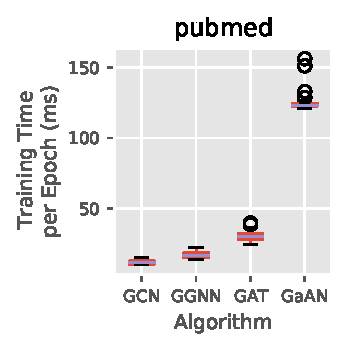
\includegraphics[height=4cm]{figs/experiments/exp_absolute_training_time_comparison_pubmed.pdf}}
    \subfloat[\texttt{aph}\label{fig:exp_absolute_training_time_amazon-photo}]{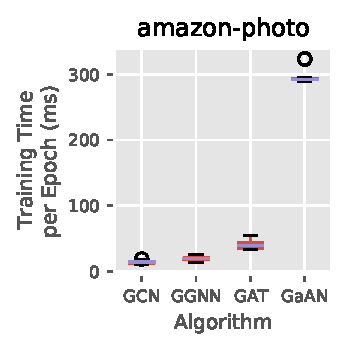
\includegraphics[height=4cm]{figs/experiments/exp_absolute_training_time_comparison_amazon-photo.pdf}}
    \subfloat[\texttt{cph}\label{fig:exp_absolute_training_time_coauthor-physics}]{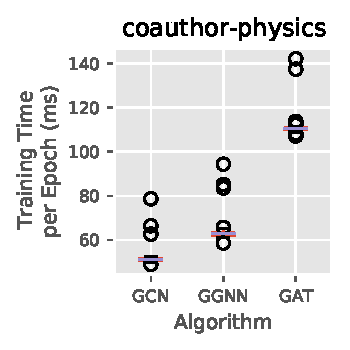
\includegraphics[height=4cm]{figs/experiments/exp_absolute_training_time_comparison_coauthor-physics.pdf}} \\
    \subfloat[\texttt{amc}\label{fig:exp_absolute_training_time_amazon-computers}]{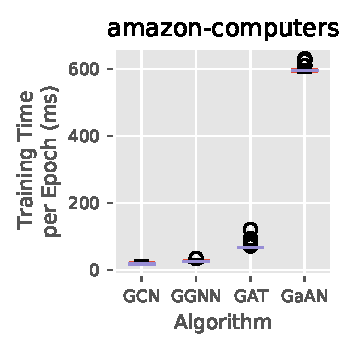
\includegraphics[height=4cm]{figs/experiments/exp_absolute_training_time_comparison_amazon-computers.pdf}}
    \subfloat[\texttt{fli}\label{fig:exp_absolute_training_time_flickr}]{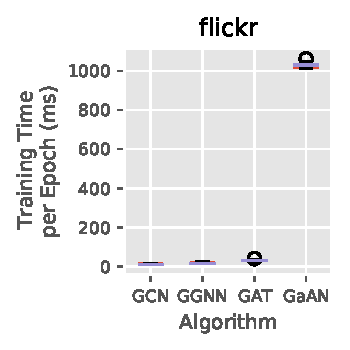
\includegraphics[height=4cm]{figs/experiments/exp_absolute_training_time_comparison_flickr.pdf}}
    \subfloat[\texttt{cam}\label{fig:exp_absolute_training_time_com-amazon}]{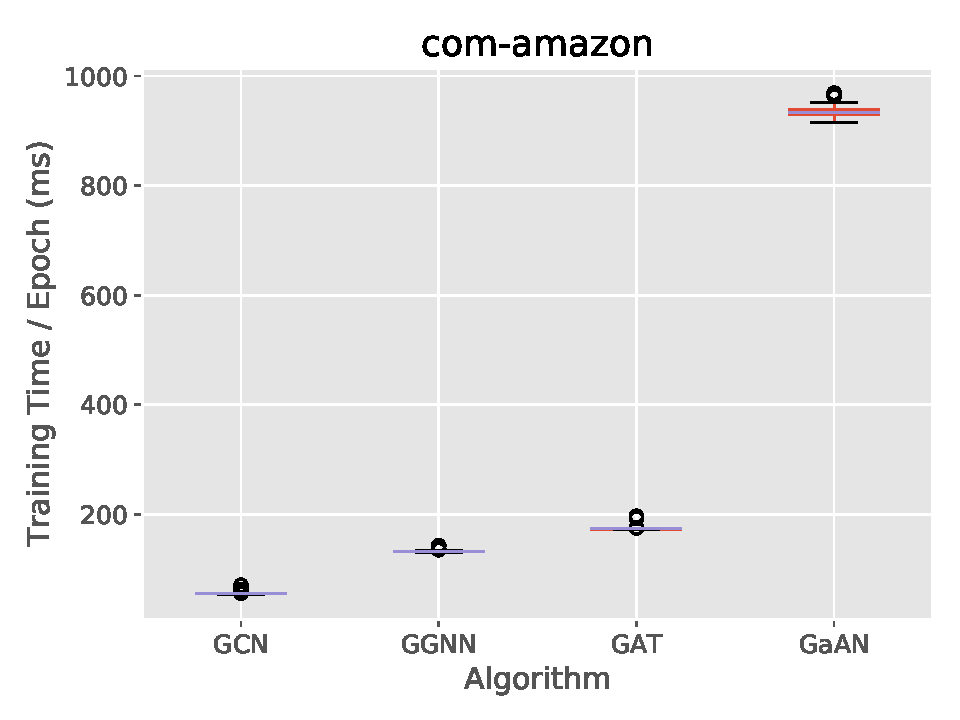
\includegraphics[height=4cm]{figs/experiments/exp_absolute_training_time_comparison_com-amazon.pdf}}
    \caption{Distribution of the wall-clock training time of 50 epoches on different datasets. GaAN crashed due to out of memory exception on the \texttt{cph} dataset.}
    \label{fig:exp_absolute_training_time}
\end{figure}

To further evaluate effects of hyper-parameters on performance, we measured the training time of each GNN with varying hyper-parameters in \figurename~\ref{fig:exp_hyperparameter_on_vertex_edge_phase_time}.

\begin{figure}[H]
    \centering
    \subfloat[GCN\label{fig:exp_hyperparameter_on_vertex_edge_phase_time_gcn}]{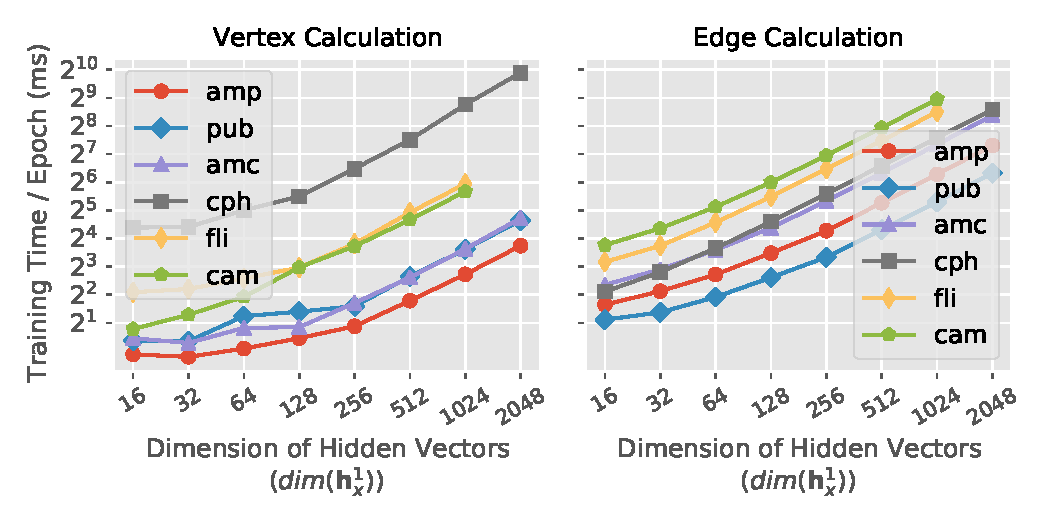
\includegraphics[height=3cm]{figs/experiments/exp_hyperparameter_on_vertex_edge_phase_time_gcn.pdf}}
    \\
    \subfloat[GGNN\label{fig:exp_hyperparameter_on_vertex_edge_phase_time_ggnn}]{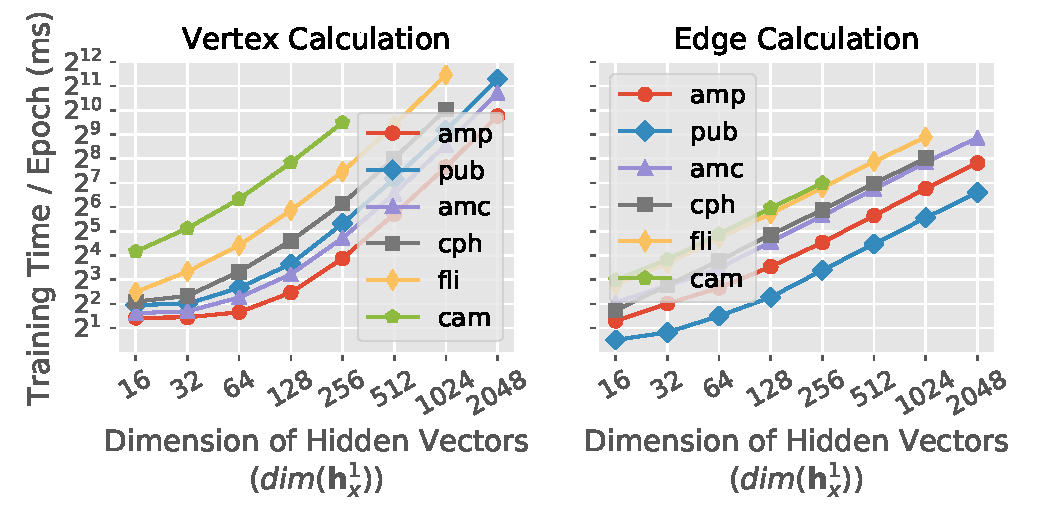
\includegraphics[height=3cm]{figs/experiments/exp_hyperparameter_on_vertex_edge_phase_time_ggnn.pdf}}
    \\
    \subfloat[GAT\label{fig:exp_hyperparameter_on_vertex_edge_phase_time_gat}]{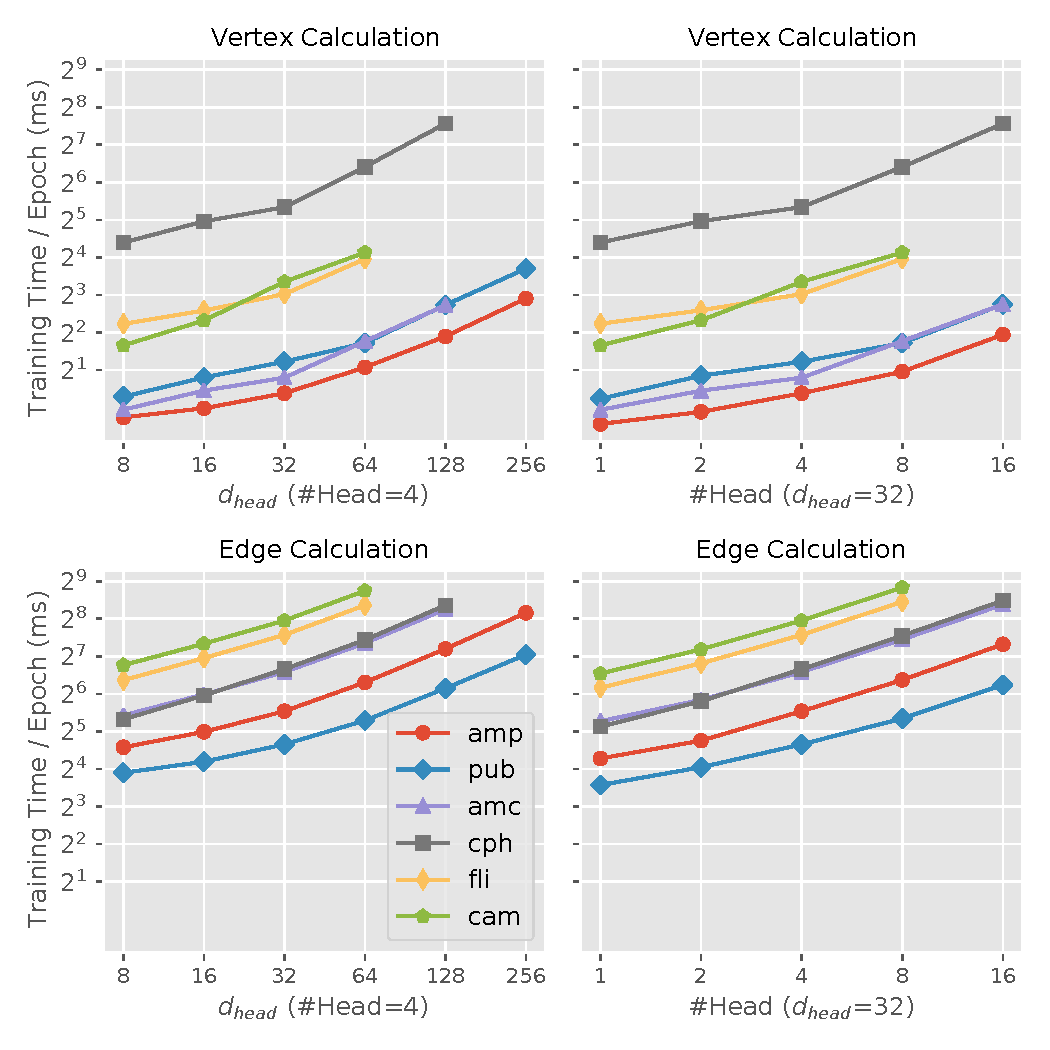
\includegraphics[height=6cm]{figs/experiments/exp_hyperparameter_on_vertex_edge_phase_time_gat.pdf}}
    \\
    \subfloat[GaAN\label{fig:exp_hyperparameter_on_vertex_edge_phase_time_gaan}]{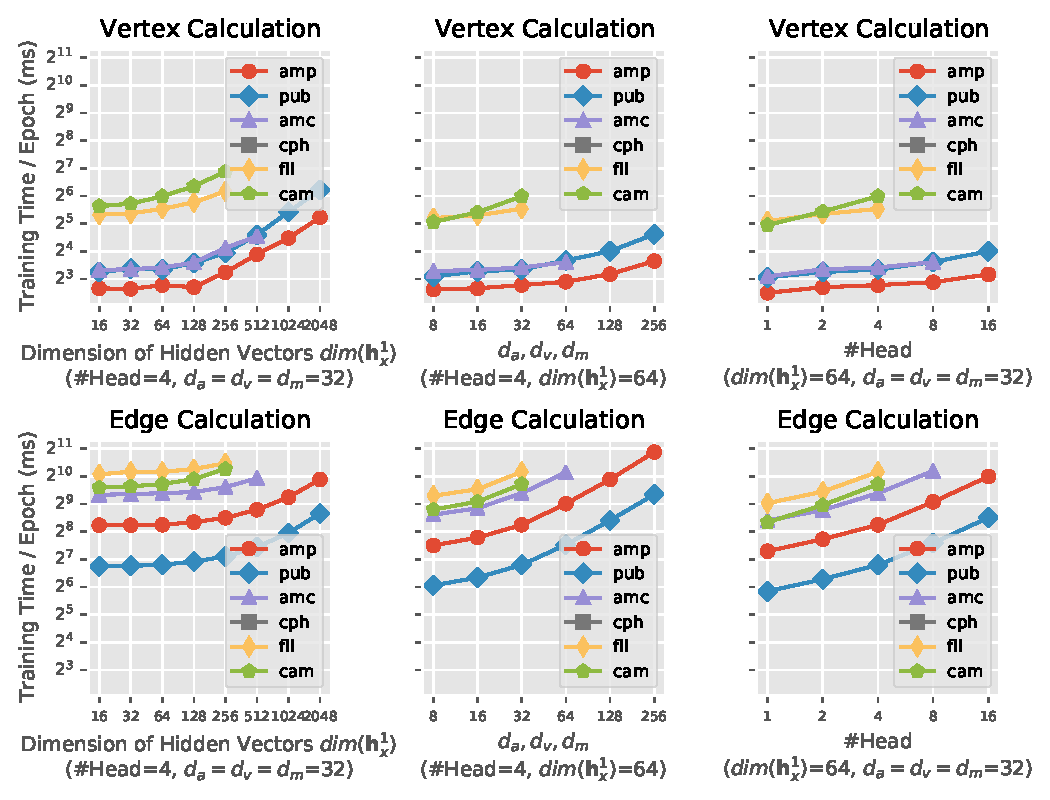
\includegraphics[height=6cm]{figs/experiments/exp_hyperparameter_on_vertex_edge_phase_time_gaan.pdf}}

    \caption{Effects of hyper-parameters on the edge/vertex calculation time.}
    \label{fig:exp_hyperparameter_on_vertex_edge_phase_time}
\end{figure}

For GCN and GGNN, $dim(\MyVec{h}^0_x)$ and $dim(\MyVec{h}^1_x)$ were solely determined by the dataset with $d^0_{in} = dim(\MyVec{h}^0_x) = dim(\MyVec{v_x})$ and $d^1_{out} = dim(\boldsymbol{h}^2_x)=\#Class$.
%
Therefore, the only modifiable hyper-parameter was the dimension of $\MyVec{h}^1_x$ that affected the dimension of output hidden vectors of the layer 0 $d^0_{out}$ and the dimension of input hidden vectors of the layer 1 $d^1_{in}$ simultaneously, i.e. $dim(\MyVec{h}^1_x)  = d^0_{out} = d^1_{in}$.
%
According to the time complexity analysis, if we fixed other hyper-parameters but only increased $dim(\boldsymbol{h}^1_x)$, the computational costs of the GNN layer 0 and the GNN layer 1 should both increase linearly with $dim(\boldsymbol{h}^1_x)$, causing the training time of the whole GNN also increasing linearly. 
%
\figurename~\ref{fig:exp_hyperparameter_on_vertex_edge_phase_time_gcn} and \figurename~\ref{fig:exp_hyperparameter_on_vertex_edge_phase_time_ggnn} show that the training time of GCN and GGNN increased linearly with $dim(\boldsymbol{h}^1_x)$ when $dim(\boldsymbol{h}^1_x)$ was big, consistent with the theoretical analysis.

For GAT, we modified the number of heads $K$ and the dimension of each head $d_{head}$ in the GAT layer 0.
%
The dimension of $\MyVec{h}^1_x$ is determined as $dim(\boldsymbol{h}^1_x) = K d_{head}$.
%
Thus, the computational costs of the GAT layer 0 and the GAT layer 1 should increase linearly with $K$ and $d_{head}$ separately. 
%
\figurename~\ref{fig:exp_hyperparameter_on_vertex_edge_phase_time_gat} confirms the theoretical analysis.

For GaAN, it is also based on the multi-head mechanism.
%
Its time complexity shoud be affected by $dim(\boldsymbol{h}^1_x)$ ($d^0_{out} = d^1_{in} = dim(\boldsymbol{h}^1_x)$), $d_a$, $d_v$, $d_m$, and the number of heads $K$.
%
\figurename~\ref{fig:exp_hyperparameter_on_vertex_edge_phase_time_gaan} demonstrates that the training time increased linearly with the hyper-parameters, except for $dim(\boldsymbol{h}^1_x)$.
As $dim(\boldsymbol{h}^1_x)$ increased, the training time increased first slightly and then linearly.
We observed similar phenomena in GCN, GGNN, and GAT:
When the values of hyper-parameters were too low, GNN training could not make full use of the computing power of the GPU.
%
When the values of hyper-parameters became high enough, training time increased linearly, supporting the time complexity analysis.

We further measured the effects of the hyper-parameters on the peak GPU memory usage in \figurename~\ref{fig:exp_hyperparameter_memory_usage}.
%
The memory usage also increased linearly as the hyper-parameters increased for all GNNs, except for GaAN on $dim(\MyVec{h}^1_x)$.
%
As the hidden vectors $\MyVec{h}^1_x$ consumed a small proportion of memory in GaAN, the growth in the memory usage was not noticeable until $dim(\boldsymbol{h}^1_x)$ was large enough.

\begin{figure}[H]
    \centering
    \subfloat[GCN]{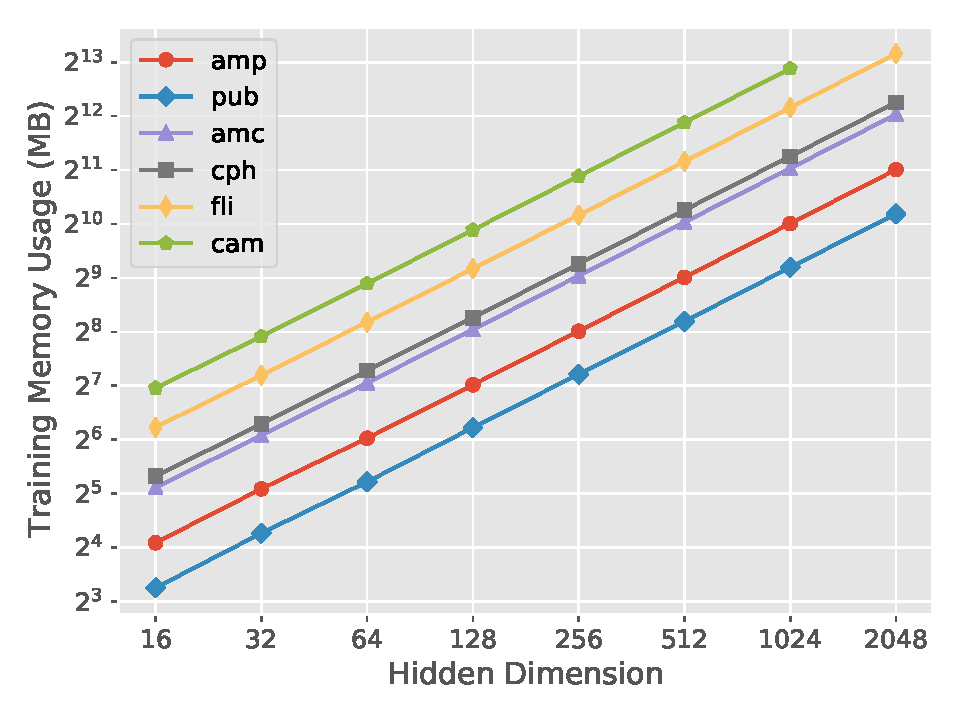
\includegraphics[height=3cm]{figs/experiments/exp_hyperparameter_on_memory_usage_gcn.pdf}}
    \subfloat[GGNN]{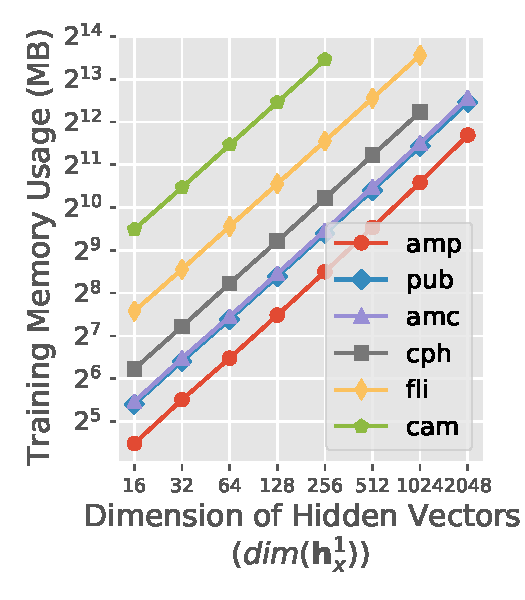
\includegraphics[height=3cm]{figs/experiments/exp_hyperparameter_on_memory_usage_ggnn.pdf}}\\
    \subfloat[GAT]{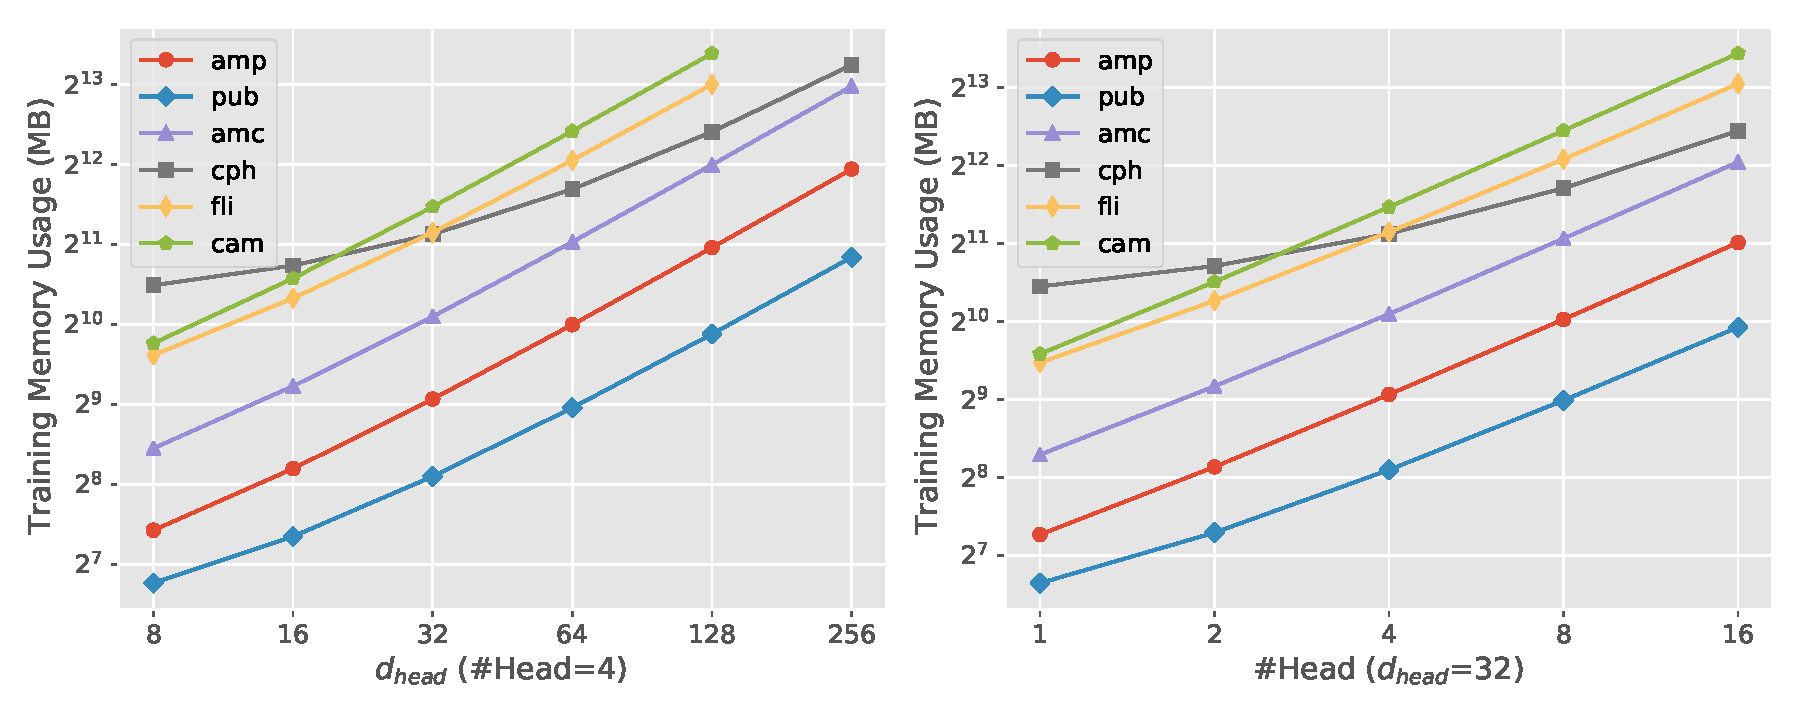
\includegraphics[height=3cm]{figs/experiments/exp_hyperparameter_on_memory_usage_gat.pdf}}\\
    \subfloat[GaAN]{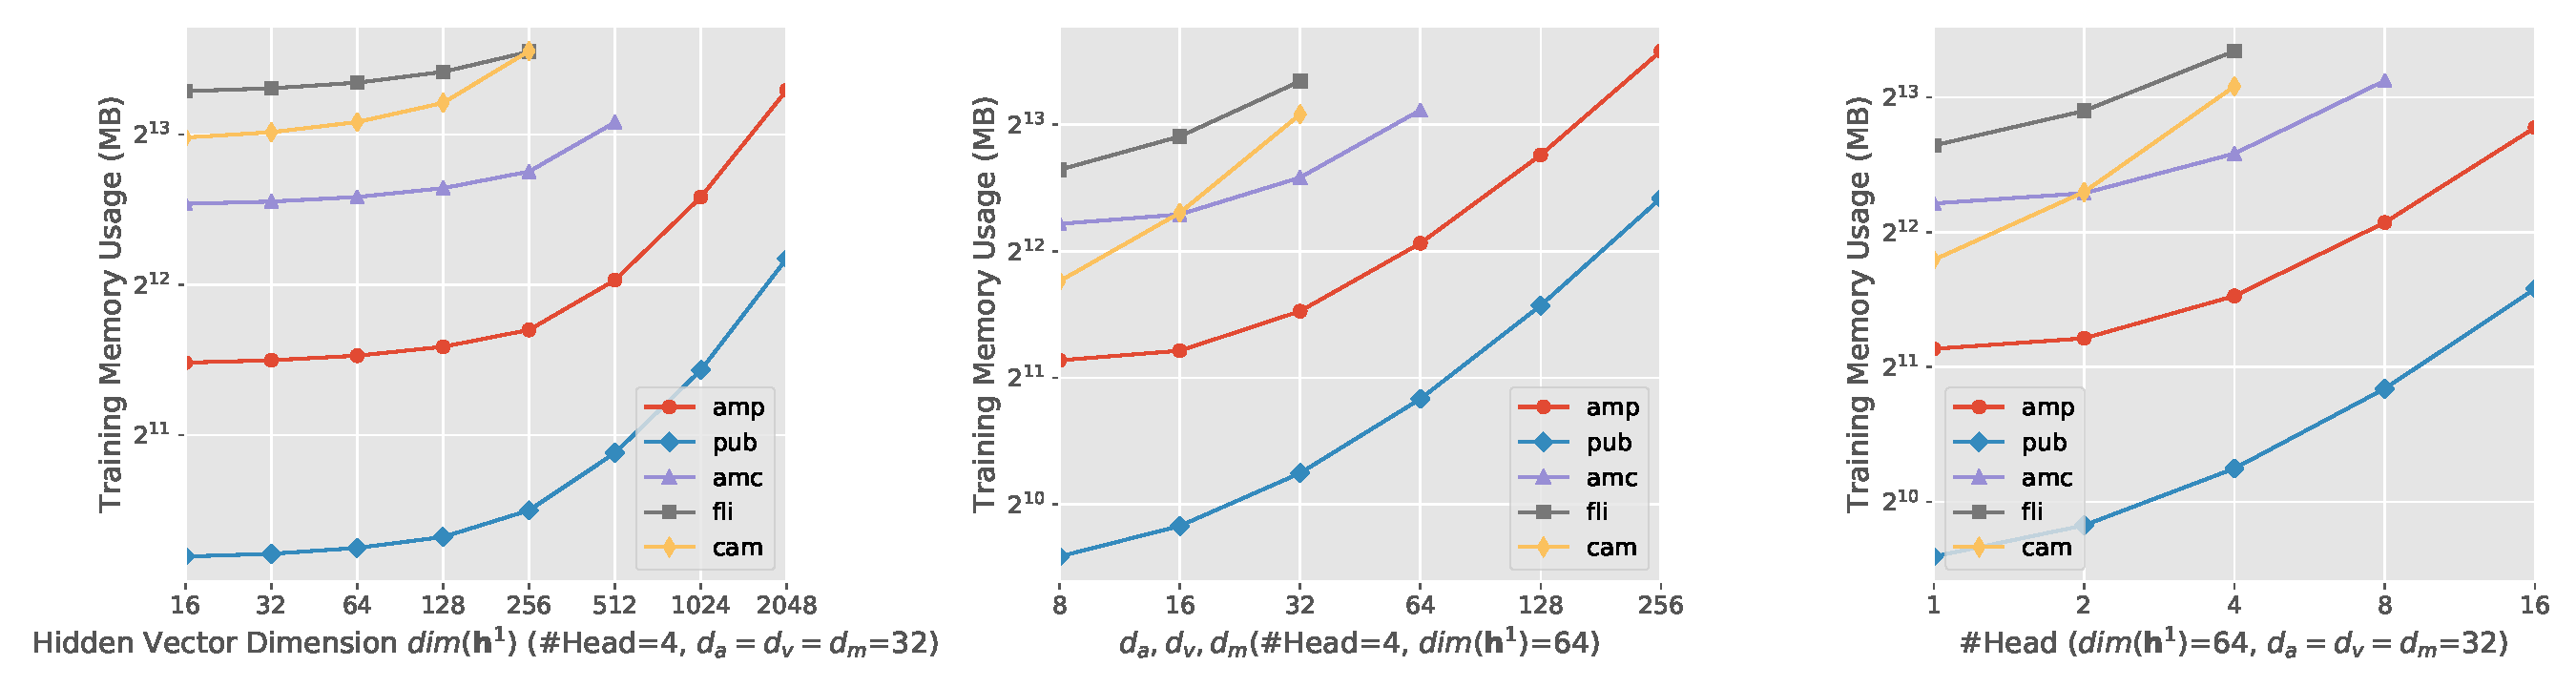
\includegraphics[height=3cm]{figs/experiments/exp_hyperparameter_on_memory_usage_gaan.pdf}}
    \caption{Effects of hyper-parameters on the peak GPU memory usage during the training, excluding the memory used by the dataset and the model parameters.}
    \label{fig:exp_hyperparameter_memory_usage}
\end{figure}

\paragraph{Summary}

The complexity analysis in \tablename~\ref{tab:gnn_overview_edge} and \tablename~\ref{tab:gnn_overview_vertex} is valid.
%
Fixing other hyper-parameters, each hyper-parameter itself affects the training time and the memory usage of a GNN Layer \emph{in a linear way}.
%
Algorithm engineers can adjust hyper-parameters according to the time complexity to avoid explosive growth in the training time and memory usage.

\subsection{Training Time Breakdown}
\label{sec:training_time_breakdown}

To find out which stage/step dominated the training time, we decomposed the training time and analyzed performance bottlenecks level by level.

\subsubsection{Layer Level}

\figurename~\ref{fig:exp_vertex_edge_cal_proportion} decomposes the training time of a GNN on the layer level.
%
The training time of each layer was the summation of the time in the forward, backward, and evaluation phases.
%
In GCN, GAT, and GaAN, the time spent on the layer 0 was much larger than the layer 1.
%
In those GNNs, the dimensions of the input/output hidden vectors in the layer 0 were much larger than the dimensions in the layer 1: $d^0_{in}=dim(\boldsymbol{v}_x)$, $d^0_{out}=d^1_{in}=64$, $d^1_{out}=\#Class$, and $dim(\boldsymbol{v}_x) \gg \#Class$.
%
For GaAN, since it required the dimensions of the input/output hidden vectors must be the same, the hyper-parameters were set to $d^0_{in}=d^0_{out}=d^1_{in}=d^1_{out}=64$ and the training time of both layers was close.

\begin{figure}[H]
    \centering
    \subfloat[GCN]{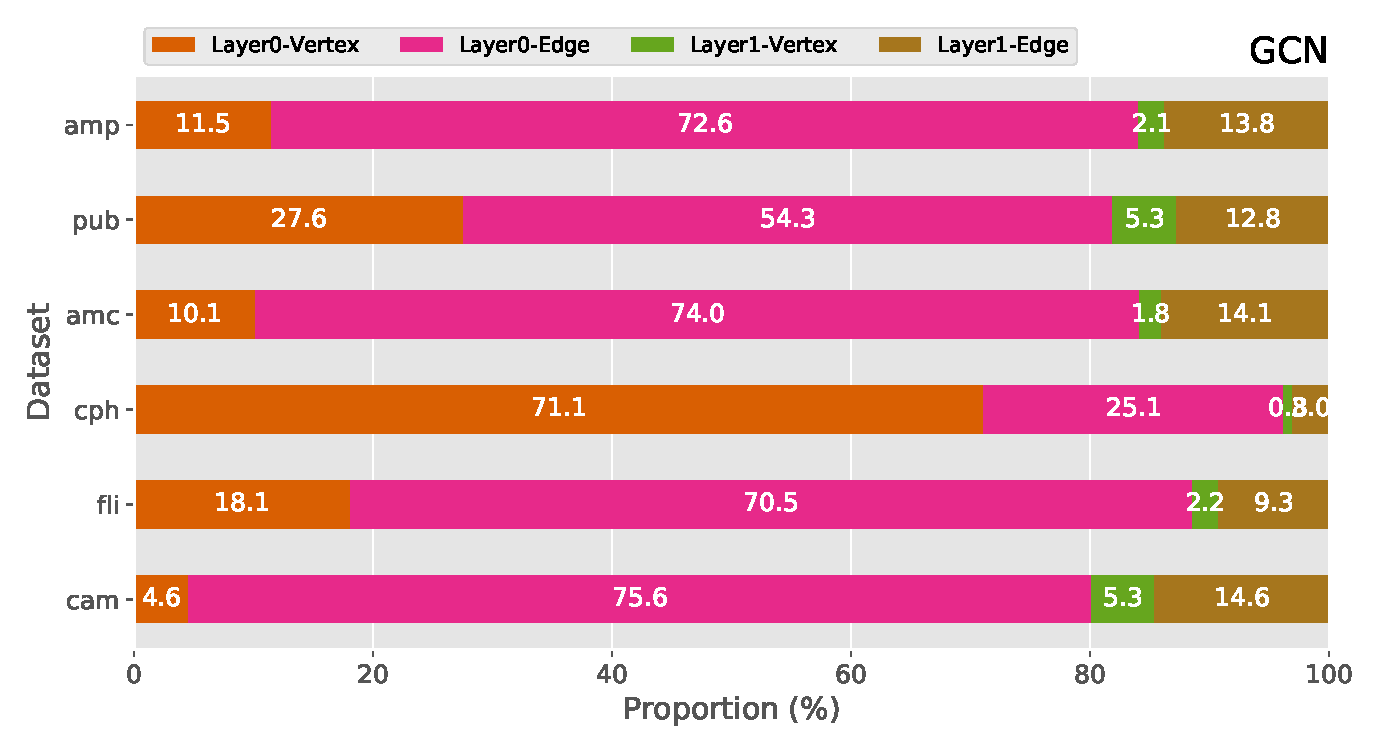
\includegraphics[height=4.6cm]{figs/experiments/exp_layer_time_proportion_gcn.pdf}}
    \subfloat[GGNN]{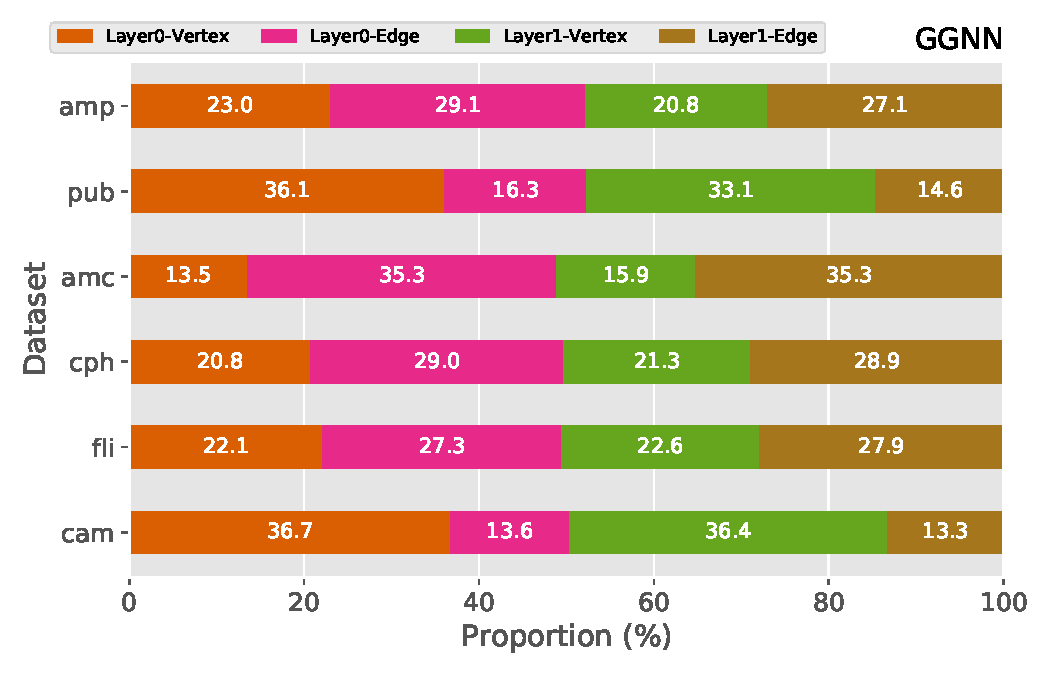
\includegraphics[height=4.6cm]{figs/experiments/exp_layer_time_proportion_ggnn.pdf}}\\
    \subfloat[GAT]{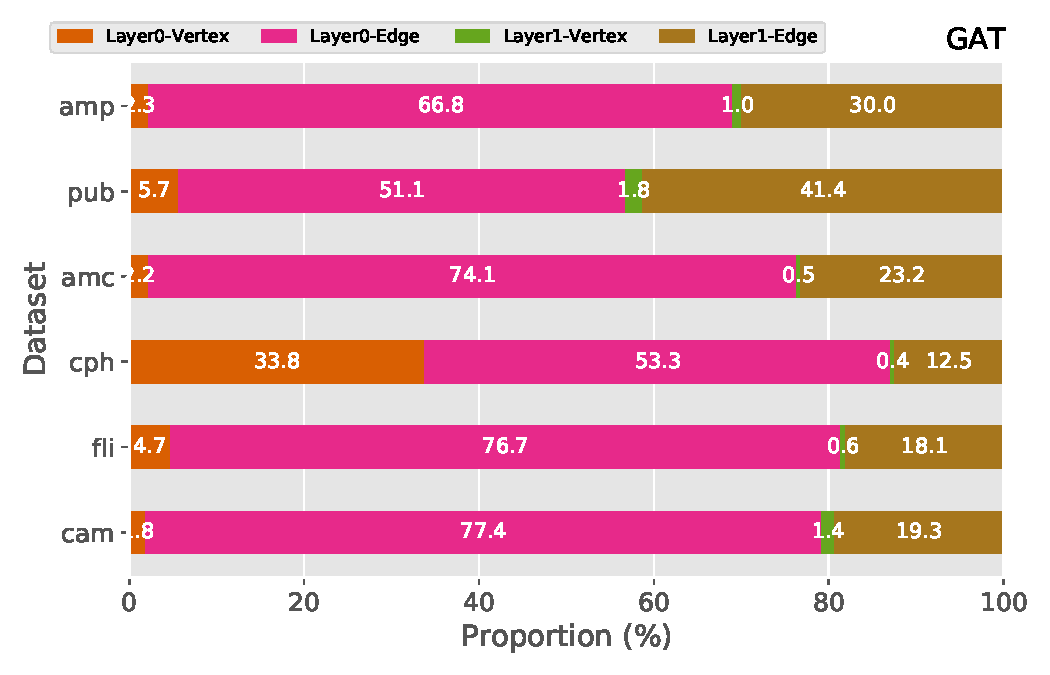
\includegraphics[height=4.6cm]{figs/experiments/exp_layer_time_proportion_gat.pdf}}
    \subfloat[GaAN]{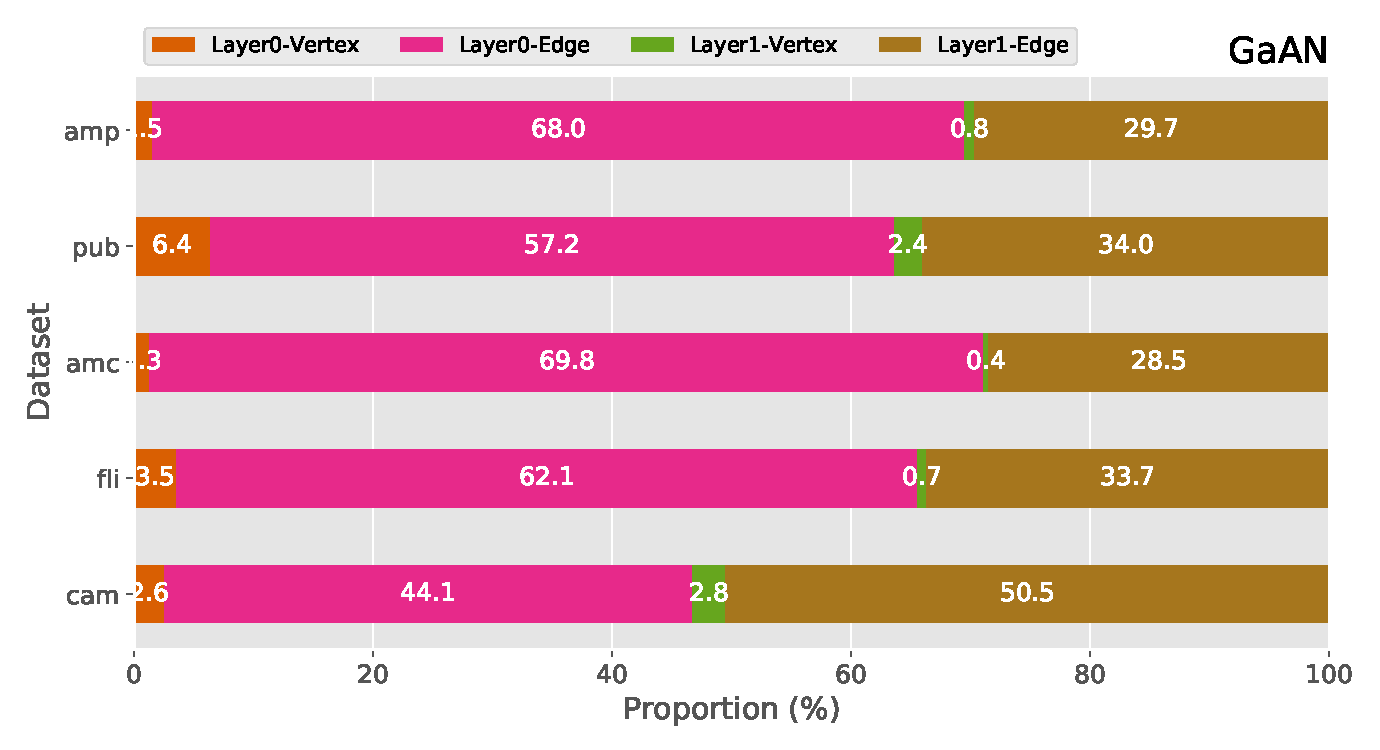
\includegraphics[height=4.6cm]{figs/experiments/exp_layer_time_proportion_gaan.pdf}}
    \caption{Training time breakdown on the layer level. The training time of each layer included the time spent on the forward, backward and evaluation phases. Each layer was further decomposed into the vertex and the edge calculation stages.}
    \label{fig:exp_vertex_edge_cal_proportion}
\end{figure}

Each GNN layer was further divided into the vertex and the edge calculation stages.
%
In \figurename~\ref{fig:exp_vertex_edge_cal_proportion}, GCN spent most of the training time on the edge calculation stage on most datasets.
%
A special case was the \texttt{cph} dataset.
%
The dimension of the input feature vectors was very high in \texttt{cph}, making the vertex calculation stage of the GCN Layer 0 spend considerable time.
%
GGNN also spent the majority of its training time on the edge calculation stage, but the high time complexity of its vertex updating function $\gamma^l$ made the proportion of the vertex calculation in the total training time much higher than the other GNNs.
%
For GAT and GaAN, due to their high edge calculation complexity, the edge calculation stage was the dominant stage.

The experimental results also indicated that the average degree of the dataset affected the proportion of the edge/vertex calculation time in the total training time.
%
For GaAN, the time spent on the vertex calculation stage exceeded the edge calculation stage on the \texttt{pub} and \texttt{cam} datasets, because the average degrees of the two datasets were low, making $|\mathcal{E}|$ and $|\mathcal{V}|$ much closer.
%
To evaluate the effects of the average degree, we generated random graphs with 50,000 vertices and average degrees ranging from 2 to 100.
%
\figurename~\ref{fig:exp_avg_degree_on_vertex_edge_cal_time} shows the training time of the four GNNs under different average degrees.
%
As the average degree increased, the training time of the edge calculation stage grew \emph{linearly}.
%
For GCN, GAT, and GaAN, the edge calculation stage dominated the entire training time even when the average degrees were small.
%
Only for GGNN that had high vertex and low edge calculation complexity, the training time of the vertex calculation stage exceeded the edge calculation stage under low average degrees ($<5$).

In summary, \emph{the edge calculation stage was the most time-consuming stage in GNN training}.
%
Improving its efficiency is the key to reduce the GNN training time.

\begin{figure}[H]
    \centering
    \subfloat[GCN]{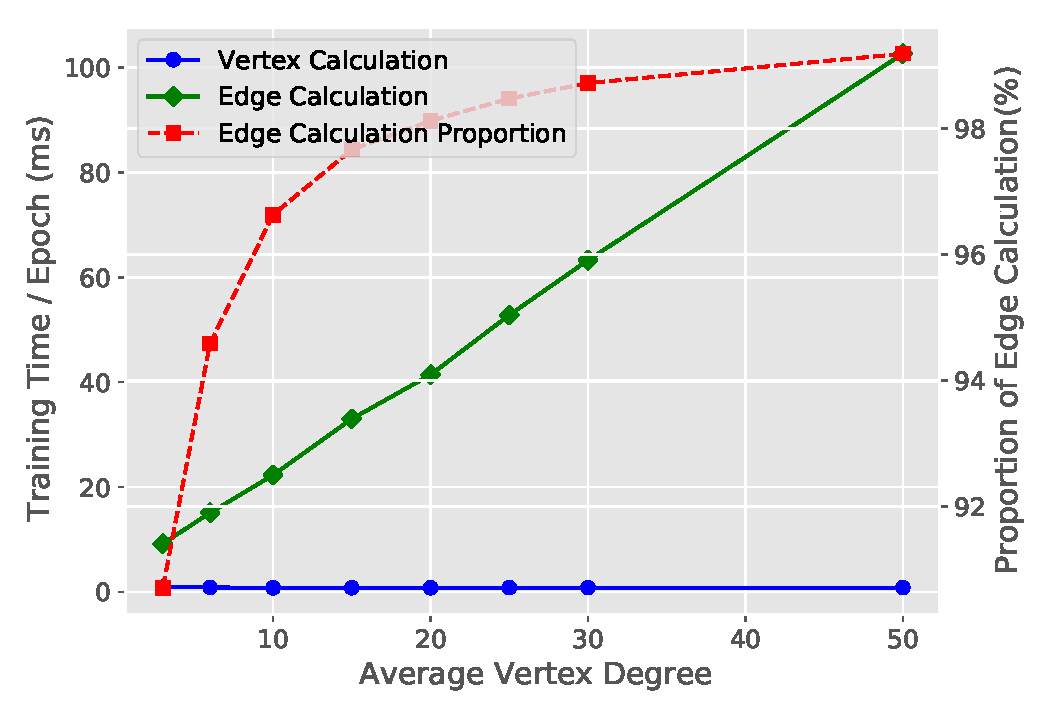
\includegraphics[height=4cm]{figs/experiments/exp_avg_degree_on_vertex_edge_cal_time_gcn.pdf}}
    \subfloat[GGNN]{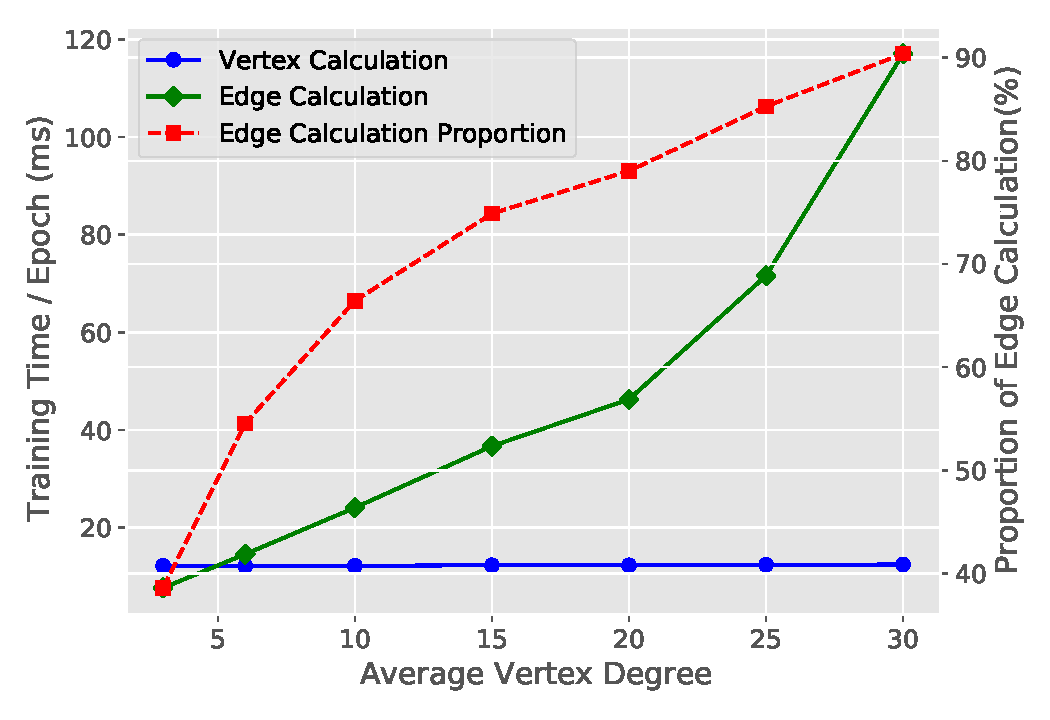
\includegraphics[height=4cm]{figs/experiments/exp_avg_degree_on_vertex_edge_cal_time_ggnn.pdf}}\\
    \subfloat[GAT]{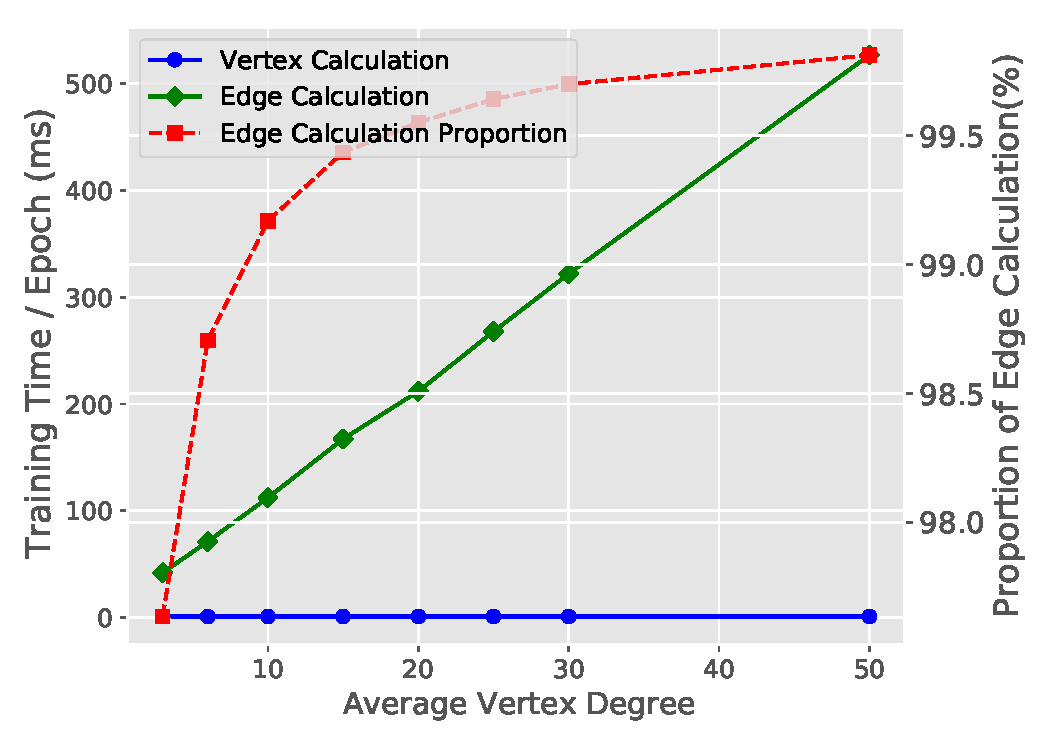
\includegraphics[height=4cm]{figs/experiments/exp_avg_degree_on_vertex_edge_cal_time_gat.pdf}}
    \subfloat[GaAN]{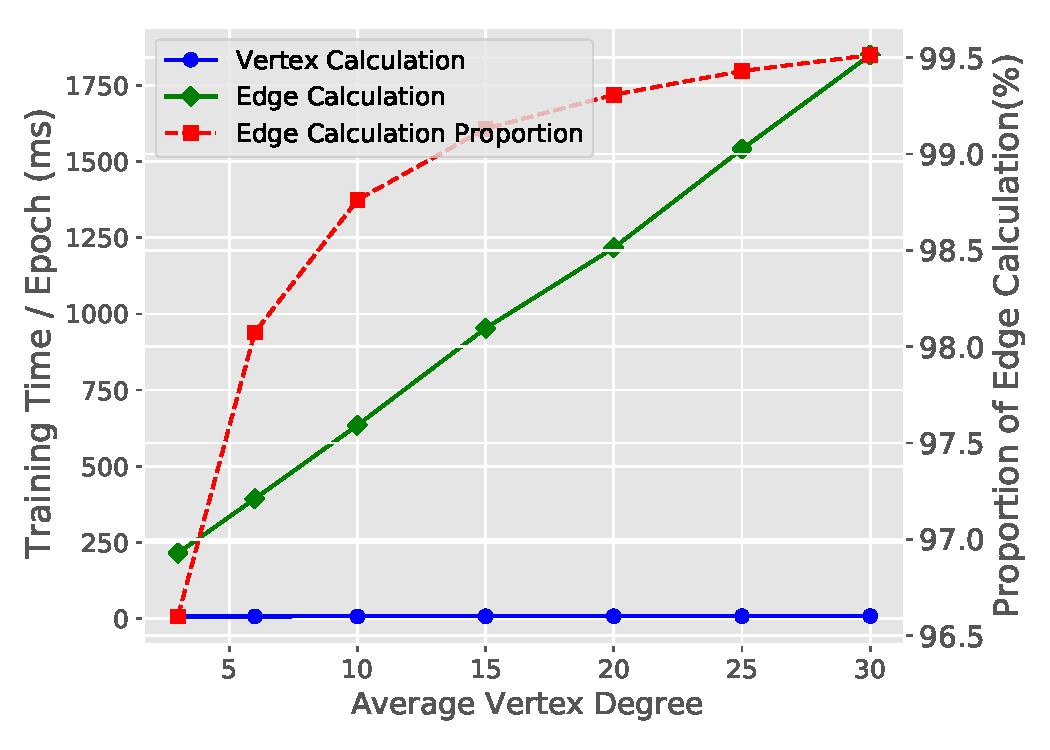
\includegraphics[height=4cm]{figs/experiments/exp_avg_degree_on_vertex_edge_cal_time_gaan.pdf}}
    \caption{Effects of the average degree on the time proportion of the edge/vertex calculation. Graphs were generated with the R-MAT generator by fixing the number of vertices as 50,000. }
    \label{fig:exp_avg_degree_on_vertex_edge_cal_time}
\end{figure}

\subsubsection{Step Level in Edge Calculation}

We further investigated the most time-consuming step of the edge calculation stage.
%
In the implementation of PyG, the edge calculation stage consists of four steps: collection, messaging, aggregation, and vector updating, as shown in \figurename~\ref{fig:steps_in_edge_calculation}.
%
The edge index is a matrix with $|\mathcal{E}|$ rows and two columns.
%
It holds the edge set of the graph.
%
The two columns of the edge index store the source and the target vertex IDs of each edge.
%
The collection step copies the hidden vectors from the previous GNN layer $\MyVec{h}^l_x$ and $\MyVec{h}^l_y$ to the both endpoints of each edge $e_{x,y}$ in the edge index, forming the parameter tensor $[\MyVec{h}^l_x, \MyVec{h}^l_{y}, \MyVec{e}_{x,y}]$ of the messaging function $\phi^l$.
%
This step only involves data movement.
%
The messaging step calls the messaging function $\phi^l$ on all edges to get message vectors $\MyVec{m}^l_{x,y}$.
%
The aggregation step aggregates the message vectors with the same target vertex into an aggregated vector $\MyVec{s}^l_x$.
%
The vector updating step is optional.
%
It performs an additional transformation on the aggregated vectors (for example, adding the bias in GCN).

\begin{figure}[H]
    \centering
    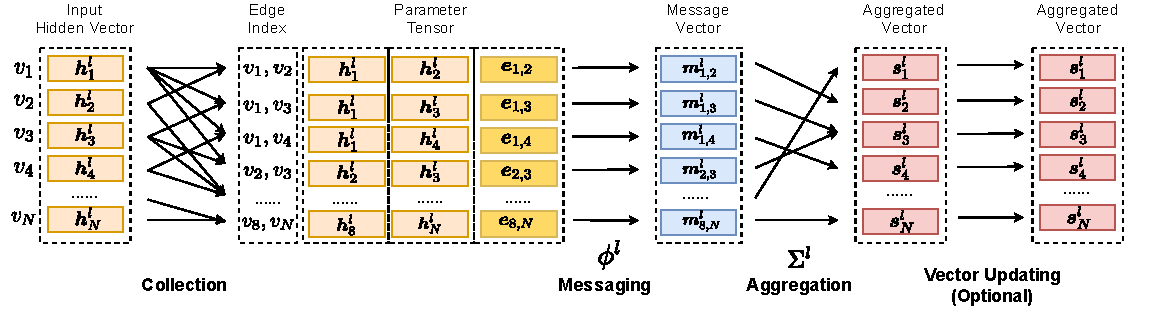
\includegraphics[width=1\columnwidth]{figs/illustration/steps_in_edge_calculation.pdf}
    \caption{Step decomposition of the edge calculation stage of the GNN layer $l$.}
    \label{fig:steps_in_edge_calculation}
\end{figure}

We decomposed the execution time of the edge calculation stage in \figurename~\ref{fig:exp_edge_calc_decomposition}.
%
In each GNN, the proportions of the four steps were rather stable, rarely affected by datasets. 
%
For GAT and GaAN with the high edge calculation complexity, the messaging step consumed most of the training time. 
%
For GCN and GGNN with the low edge complexity, the proportions of the steps were close. 
%
Since the messaging function $\phi^l$ of GGNN used the pre-computed $\MyVec{\hat{h}}^l_y$ as the message vector directly, the time spent on the messaging step of GGNN was negligible.
%
Although the collecting step did not conduct any computation and only involved data movement, it occupied noticeable execution time in the four GNNs.

The results indicate that \emph{the performance bottlenecks of the edge calculation stage depend on the complexity of the messaging function $\phi^l$}.
%
When the time complexity of $\phi^l$ is high, the messaging step is the performance bottleneck.
%
Optimizing the implementation of $\phi$ can significantly reduce training time.
%
Otherwise, the collection and the aggregation steps are performance bottlenecks.
%
Improving the efficiency of the two steps can benefit all GNNs.

\begin{figure}[H]
    \centering
    \subfloat[GCN]{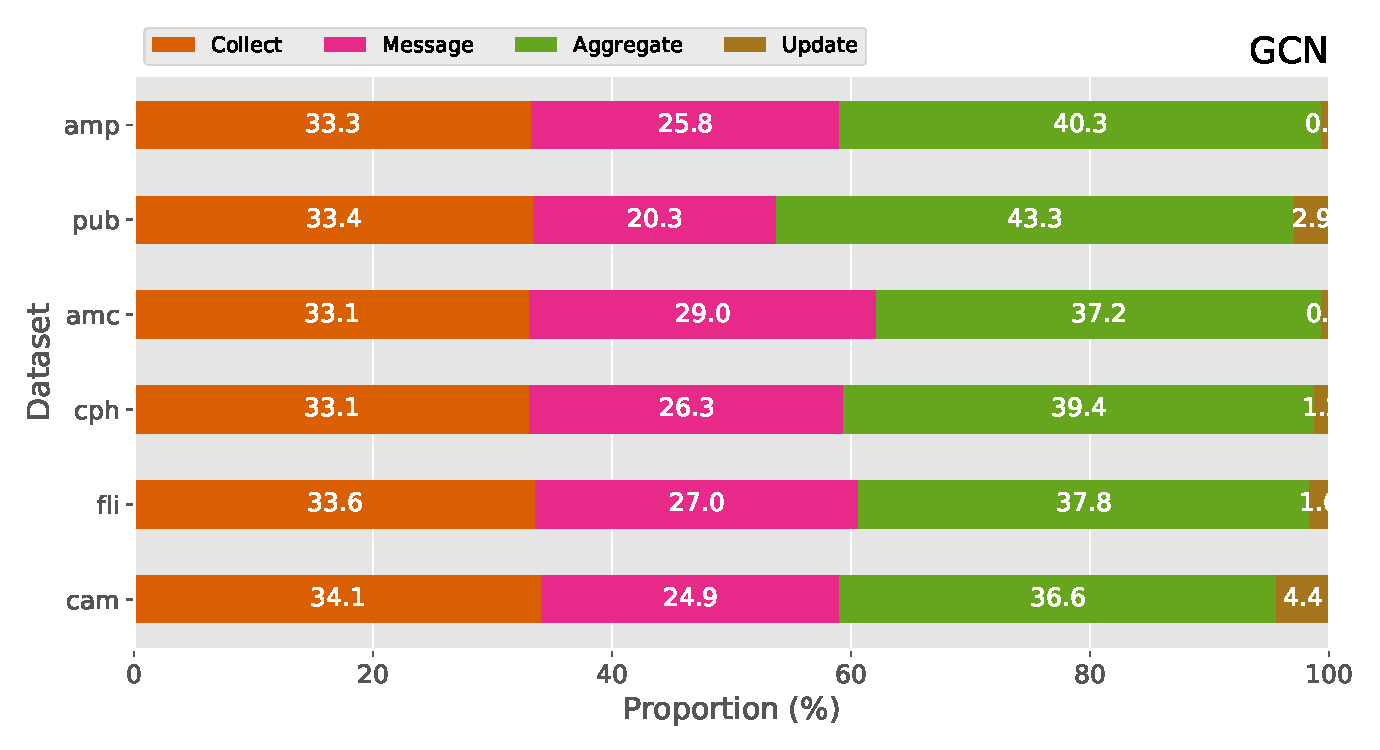
\includegraphics[height=4cm]{figs/experiments/exp_edge_calc_decomposition_gcn.pdf}}
    \subfloat[GGNN]{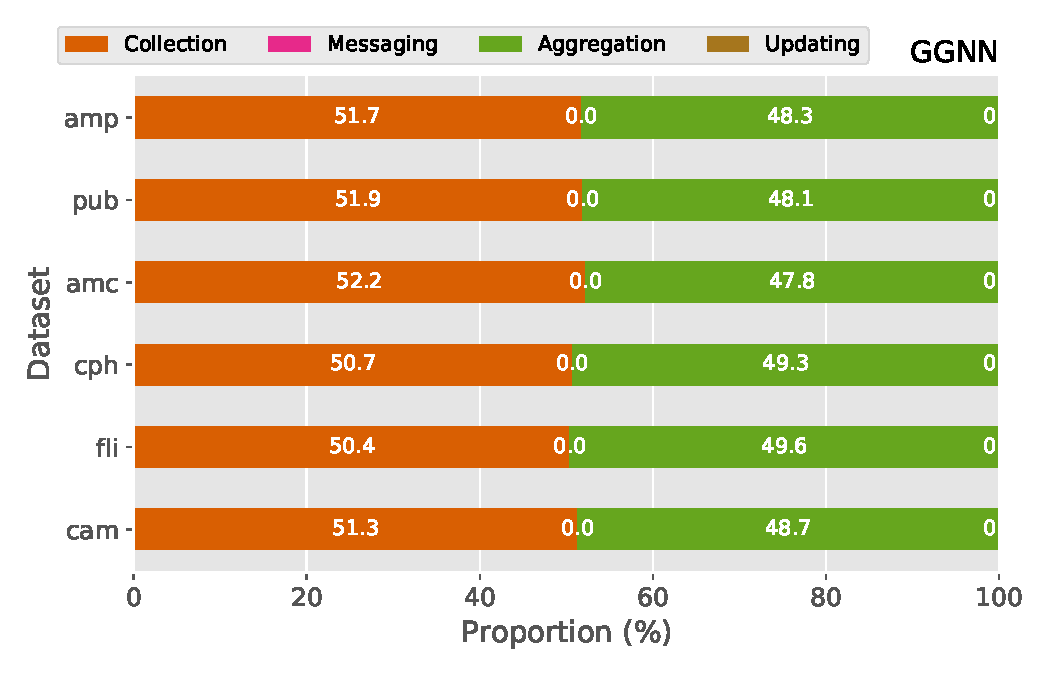
\includegraphics[height=4cm]{figs/experiments/exp_edge_calc_decomposition_ggnn.pdf}}\\
    \subfloat[GAT]{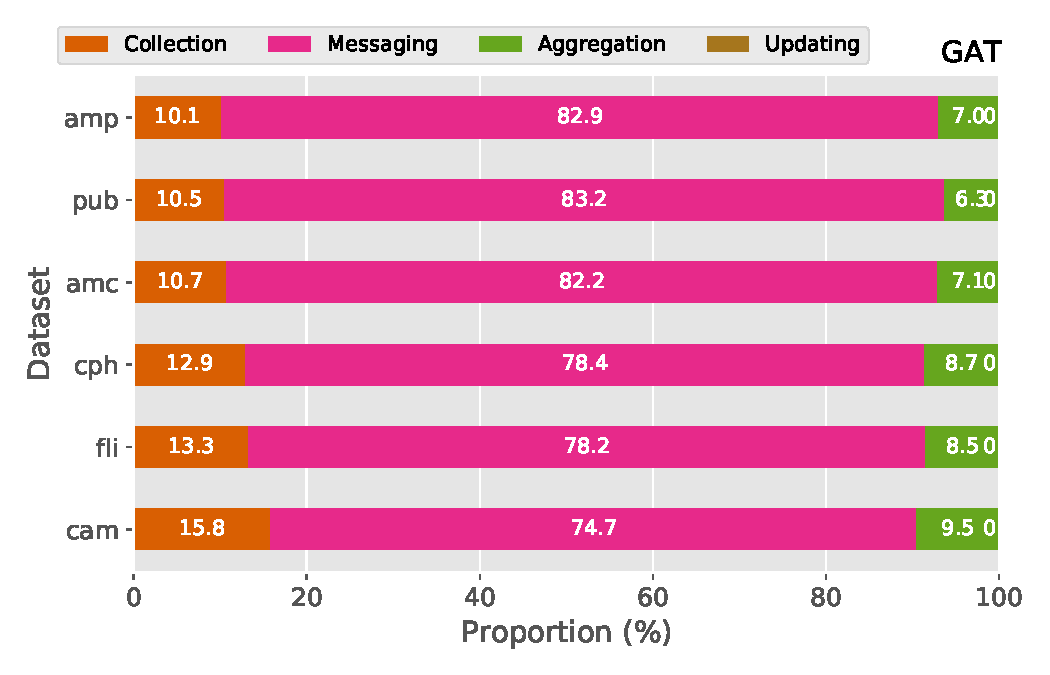
\includegraphics[height=4cm]{figs/experiments/exp_edge_calc_decomposition_gat.pdf}}
    \subfloat[GaAN]{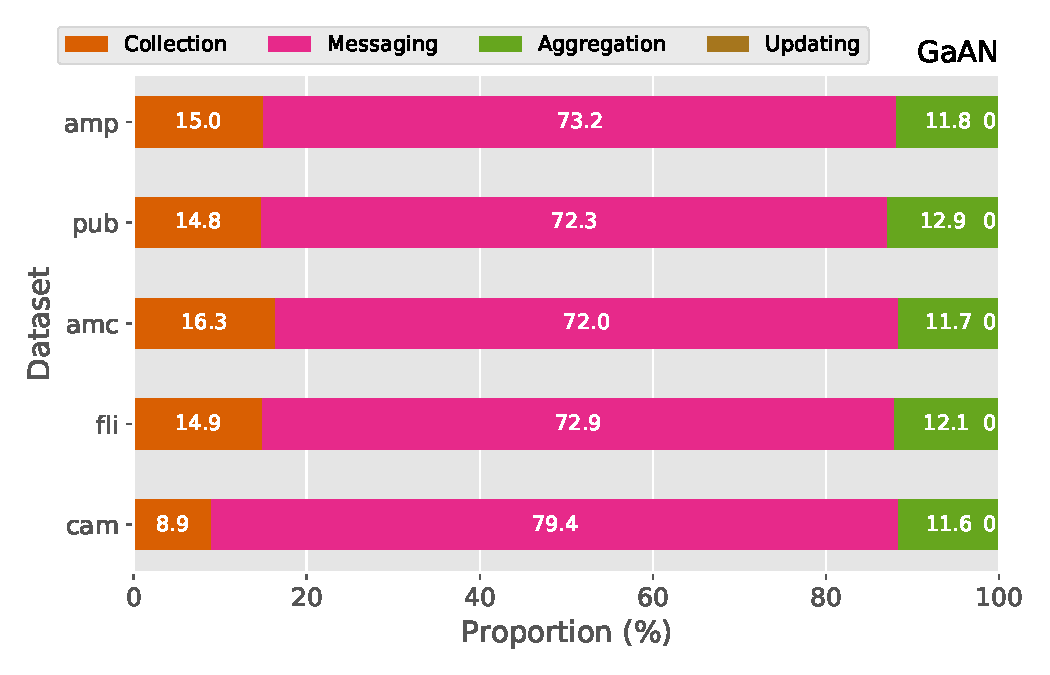
\includegraphics[height=4cm]{figs/experiments/exp_edge_calc_decomposition_gaan.pdf}}
    \caption{Training time breakdown of the edge calculation stage.}
    \label{fig:exp_edge_calc_decomposition}
\end{figure}

\subsubsection{Operator Level}

The functions $\phi$, $\Sigma$ and $\gamma$ in the edge and vertex calculation stages are made up of a series of basic operators implemented on the GPU side, such as the matrix multiplication \texttt{mm}, the elementwise multiplication \texttt{mul} and the index-based selection \texttt{index\_select}.
%
\figurename~\ref{fig:exp_top_basic_ops} shows the top-5 time-consuming basic operators in each GNN, averaged over all datasets.

\begin{figure}[H]
    \centering
    \subfloat[GCN]{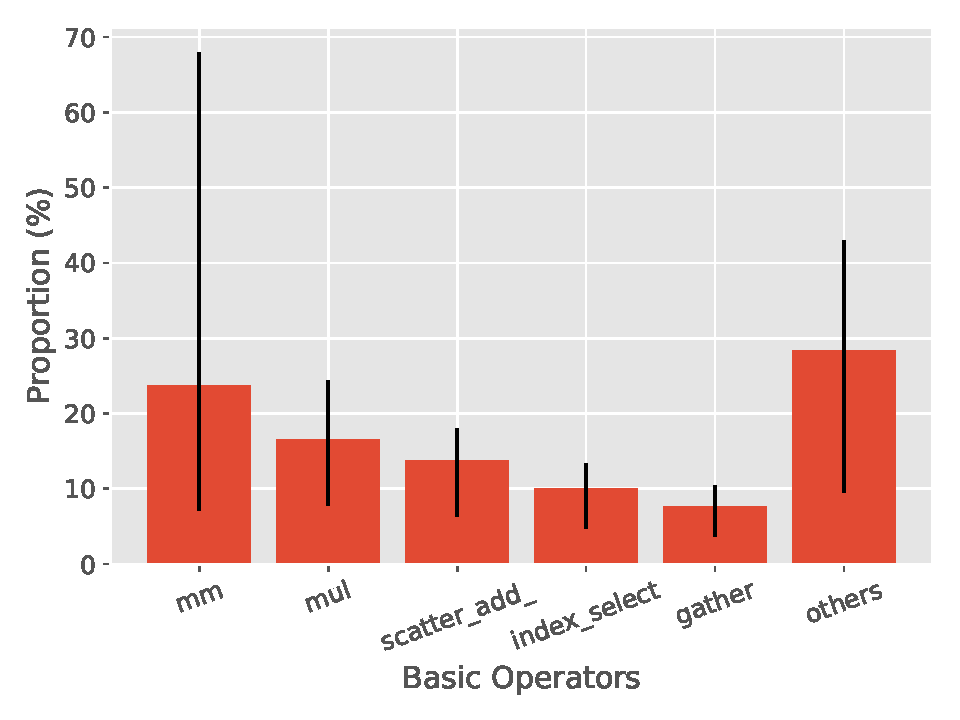
\includegraphics[height=4cm]{figs/experiments/exp_top_basic_ops_gcn.pdf}}
    \subfloat[GGNN]{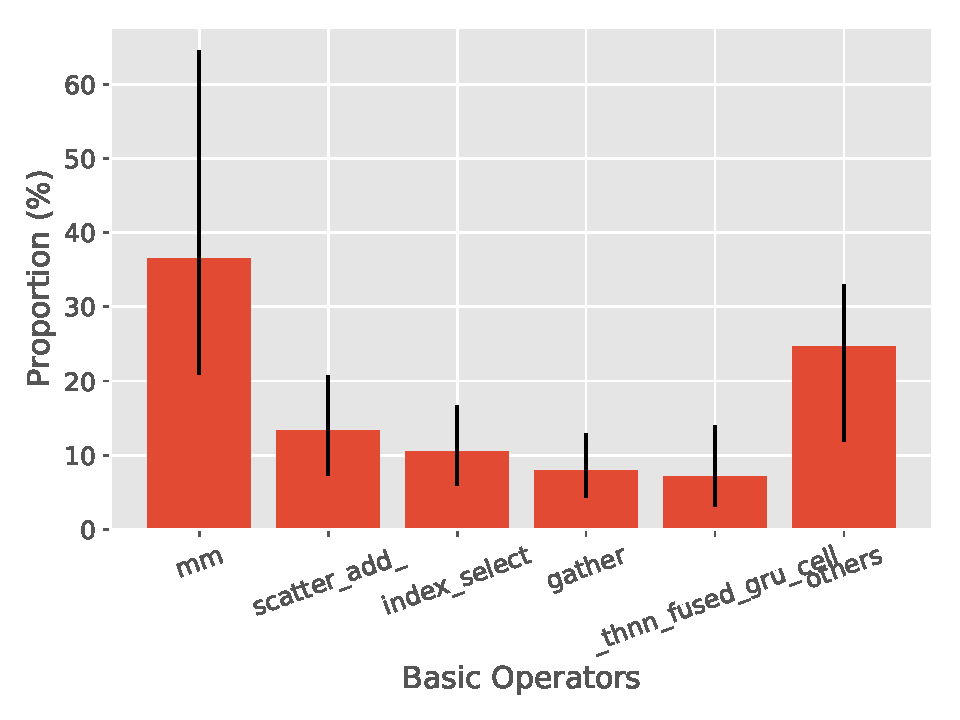
\includegraphics[height=4cm]{figs/experiments/exp_top_basic_ops_ggnn.pdf}}\\
    \subfloat[GAT]{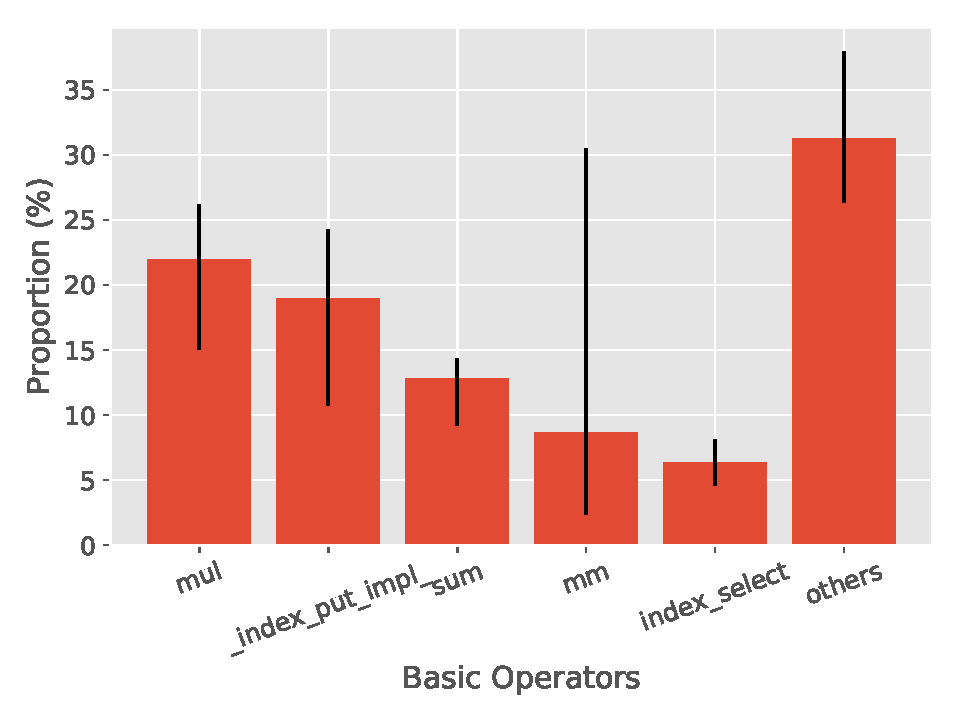
\includegraphics[height=4cm]{figs/experiments/exp_top_basic_ops_gat.pdf}}
    \subfloat[GaAN]{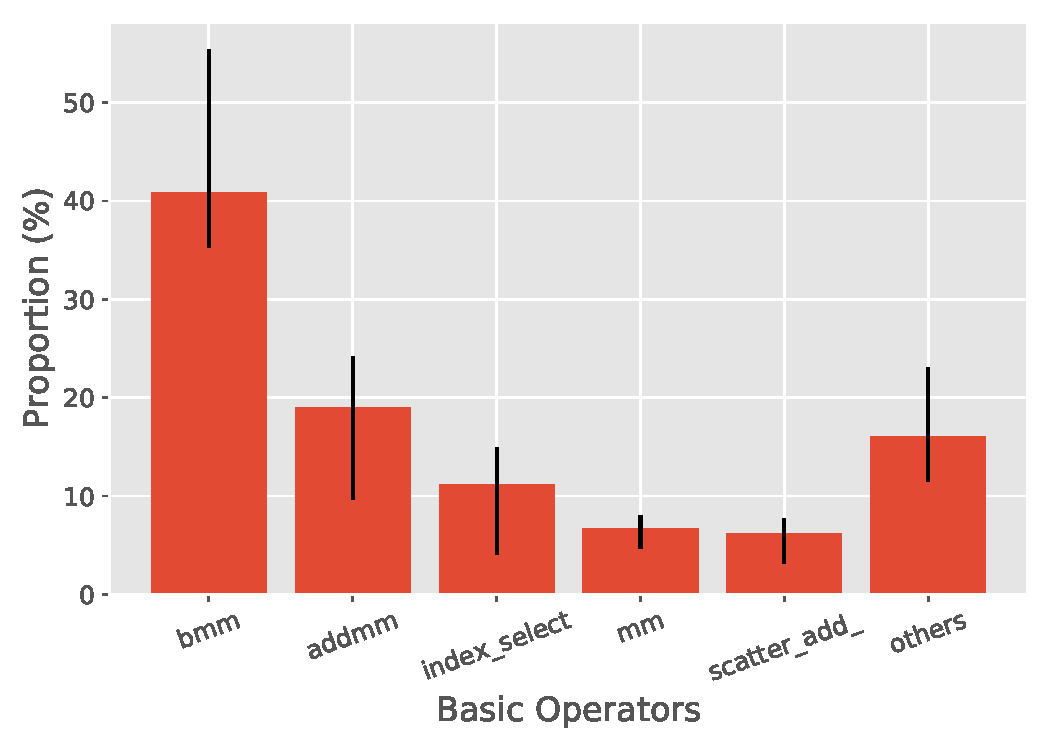
\includegraphics[height=4cm]{figs/experiments/exp_top_basic_ops_gaan.pdf}}
    \caption{Top 5 time-consuming basic operators of typical GNNs. The time proportion of each basic operator was averaged over all datasets with the error bar indicating the maximum and the minimum.}
    \label{fig:exp_top_basic_ops}
\end{figure}

\paragraph{GCN}
%
The most time-consuming basic operator was the matrix multiplication \texttt{mm} used in the vertex updating function $\gamma$.
%
The elementwise multiplication \texttt{mul} used in the messaging function $\phi$ was also time-consuming.
%
The other three operators were used in the edge calculation stage: \texttt{scatter\_add\_} for the aggregation step in the forward phase, \texttt{gather} for the aggregation step in the backward phase, and \texttt{index\_select} for the collection step.
%
For GCN, the basic operators related to the edge calculation stage consumed the majority of the training time.

\paragraph{GGNN}
%
The top basic operator was \texttt{mm} used in the vertex updating function $\gamma$.
%
Due to its high time complexity, the proportion of \texttt{mm} was much higher than the other operators.
%
The \texttt{thnn\_fused\_gru\_cell} operator was used in the backward phase of $\gamma$.
%
The other three operators were used in the edge calculation stage.

\paragraph{GAT}
%
All the top basic operators except for \texttt{mm} were related to the edge calculation stage.
%
The \texttt{mm} operator was used in the vertex updating function $\gamma$.

\paragraph{GaAN}
%
The top basic operator was \texttt{bmm} used in the messaging function $\phi$.
%
The \texttt{addmm} operator and the \texttt{mm} operator were used in both the vertex and the edge calculation stages, where the edge calculation stage was dominant.

The most time-consuming operators in the four GNNs were the matrix multiplication \texttt{mm} and the elementwise multiplication \texttt{mul}, \emph{making GNN training suitable for GPUs}.
%
Although the aggregation step in the edge calculation stage was relatively simple (like sum and mean), the related operators--\texttt{scatter\_add} and \texttt{gather}--still consumed a certain amount of the time.
%
The two operators had to synchronize between hardware threads to avoid updating the same aggregated vector at the same time.
%
They also conducted non-regular memory access with the access pattern determined by the edge set dynamically.
%
For GPUs, they were less efficient than \texttt{mm}.
%
The index-based selection operator \texttt{index\_select} used in the collection step consumed about 10\% of the training time in all GNNs.
%
Improving the efficiency of \texttt{scatter\_add}/\texttt{gather}/\texttt{index\_select} can benefit all kinds of GNNs.

\paragraph{Summary of Training Time Breakdown}
%
The GNN training was suitable for GPUs.
%
\emph{The edge calculation stage was the main performance bottleneck in most cases}, except for training GNNs with high vertex calculation complexity on low-average-degree graphs.
%
The performance bottleneck in the edge calculation stage depended on the time complexity of the messaging function $\phi$.
%
If the time complexity of $\phi$ was {high}, {$\phi$} dominated the training time of the edge calculation stage.
%
Optimizations should focus on improving its efficiency.
%
Otherwise, the {collection step} and the {aggregation step} dominated the training time.
%
The collection step suffered from lots of data movement.
%
The aggregation step suffered from data synchronization and non-regular data access.

\subsection{Memory Usage Analysis}
\label{sec:memory_usage_analysis}

During the GNN training, we stored all data (including datasets and intermediate results) in the on-chip memory of the GPU.
%
Compared with the main memory on the host side (90 GB), the capacity of the GPU memory (16 GB) was very limited.
%
\emph{The GPU memory capacity limited the scales of the graphs that it could handle}.
%
For example, GaAN was unable to train on the \texttt{cph} dataset due to the out of memory exception.

\figurename~\ref{fig:exp_memory_usage_stage_amp} shows the peak memory usage of each phase during the GNN training on the \texttt{amp} dataset.
%
The trends on the other datasets were similar.
%
\emph{The GNN training achieved its peak memory usage in the forward and the backward phases}.
%
The forward phase generated lots of intermediate results.
%
Some key intermediate results were cached for the gradient calculation in the backward phase, increasing memory usage.
%
For example, \figurename~\ref{fig:ggnn_vertex_func_computation_graph} shows the computation graph of the vertex updating function $\gamma^l$ of GGNN.
%
Each operator in the computation graph generated an intermediate tensor.
%
Some key intermediate tensors are cached.
%
The cached tensors were the main source of memory usage in the loss phase.
%
By the end of the backward phase, the cached tensors were released.
%
Since the evaluation phase did not have to calculate the gradients, it did not cache intermediate tensors.
%
Its memory usage declined sharply.

\begin{figure}[H]
    \centering
    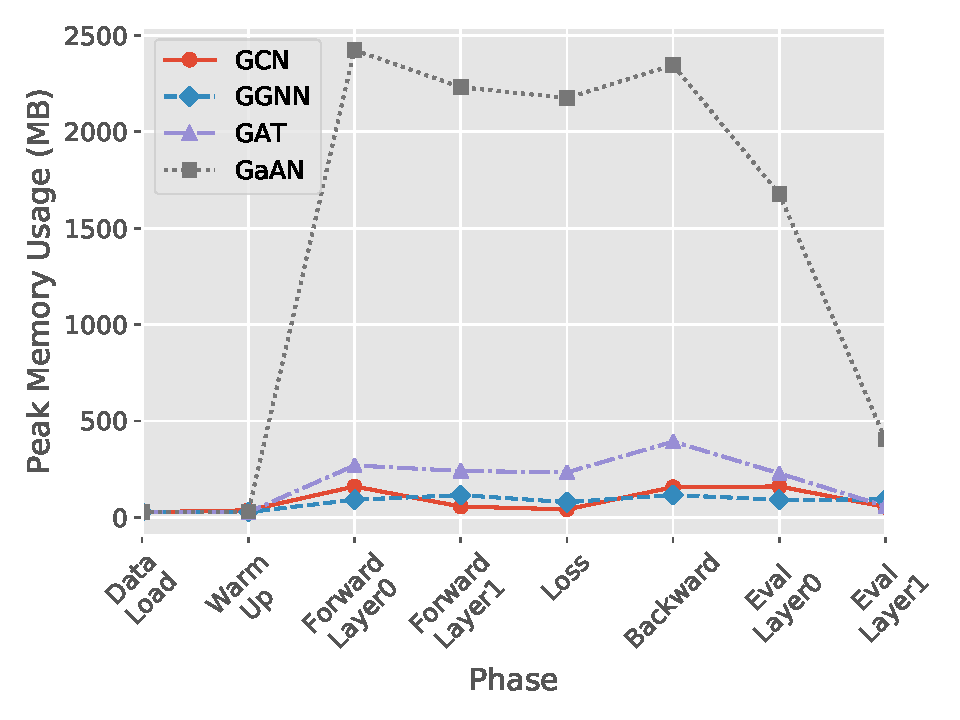
\includegraphics[height=5cm]{figs/experiments/exp_memory_usage_stage_amp.pdf}
    \caption{Memory usage of each phase during the GNN training. Dataset: \texttt{amp}.}
    \label{fig:exp_memory_usage_stage_amp}
\end{figure}

\begin{figure}[H]
    \centering
    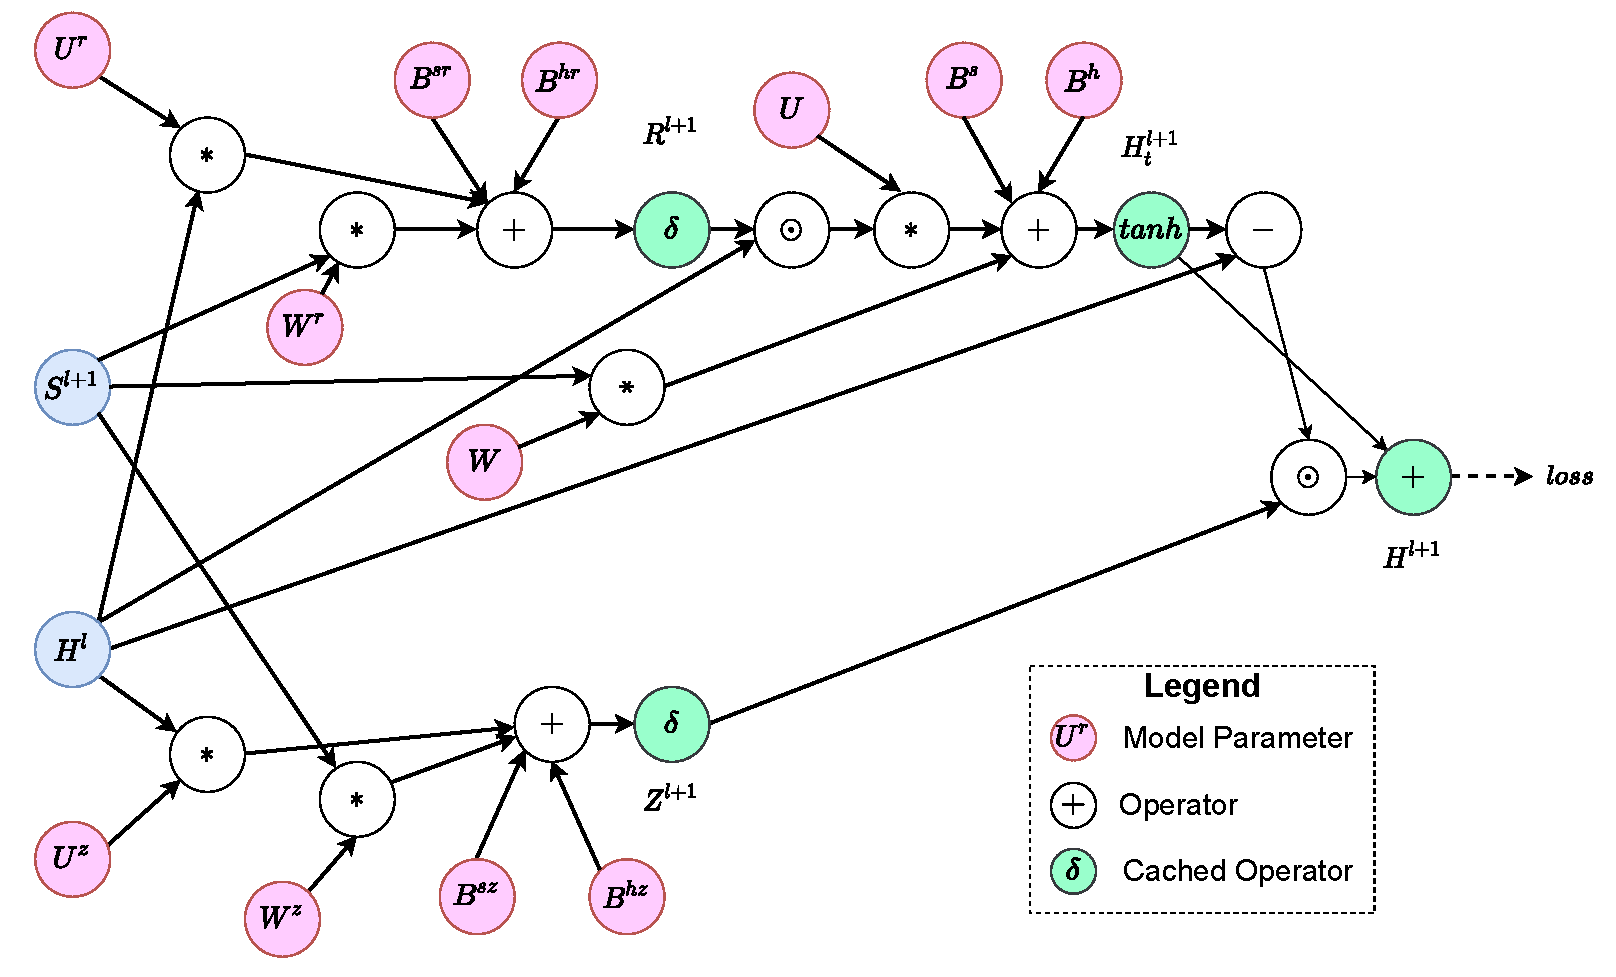
\includegraphics[width=0.7\columnwidth]{figs/illustration/ggnn_vertex_func_computation_graph.pdf}
    \caption{Computation graph of the vertex updating function $\gamma$ of GGNN.}
    \label{fig:ggnn_vertex_func_computation_graph}
\end{figure}

The peak memory usage during the GNN training far exceeded the size of the dataset itself.
%
We defined the \emph{memory expansion ratio} (MER) as the ratio of the peak memory usage during the training to the memory usage after loading the dataset.
%
\figurename~\ref{fig:exp_memory_expansion_ratio} compares MER of different GNNs.
%
GCN had the lowest MER (up to 15) while GaAN had the highest MER (up to 104).
%
\emph{The high MERs limited the data scalability of GNNs}, making GPUs unable to handle big graphs.
%
\figurename~\ref{fig:exp_memory_expansion_ratio} also indicates that the same GNN had different MERs for different datasets.
%
Two characteristics of a dataset affected the MER: the dimension of the input feature vectors and the average degree of the graph.

\begin{figure}[H]
    \centering
    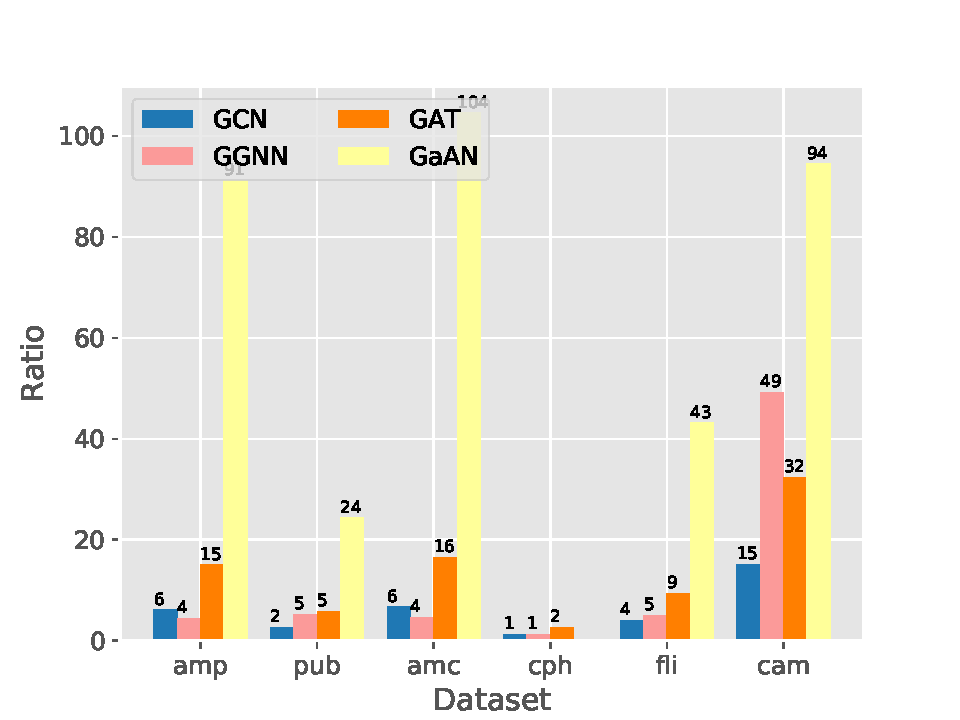
\includegraphics[width=0.5\columnwidth]{figs/experiments/exp_memory_expansion_ratio.pdf}
    \caption{Memory expansion ratios of typical GNNs.}
    \label{fig:exp_memory_expansion_ratio}
\end{figure}

To find out how the dimension of input feature vectors affected the MER, we generated random input feature vectors with different dimensions for the \texttt{cam} dataset and measured the MER in \figurename~\ref{fig:exp_memory_expension_ratio_input_feature_dimension}.
%
Under the same hyper-parameters, \emph{the MER decreased as the dimension of input feature vectors increased}.
%
When the dimension of the input feature vectors was high, the size of the dataset itself was large.
%
The size became comparable to the size of intermediate results,  making MERs low.


\begin{figure}[H]
    \centering
    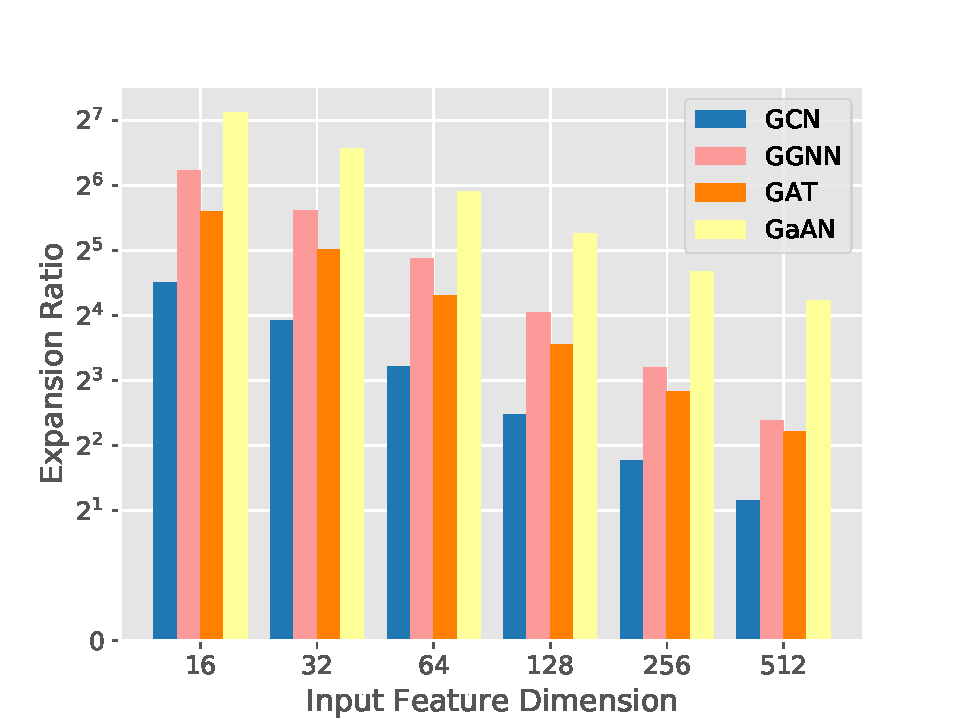
\includegraphics[height=5cm]{figs/experiments/exp_memory_expansion_ratio_input_feature_dimension_com-amazon.pdf}
    \caption{Memory expansion ratio under different dimensions of input feature vectors. Dataset: \texttt{cam}.}
    \label{fig:exp_memory_expension_ratio_input_feature_dimension}
\end{figure}

Average degrees also affected MERs by influencing the relative sizes of intermediate results from the edge and the vertex calculation stages.
%
Fixing the number of vertices $|\mathcal{V}|$, we generated random graphs with different average degrees.
%
\figurename~\ref{fig:exp_memory_expansion_ratio_input_graph_number_of_edges} shows how the memory usage changed according to the average degree.
%
As the average degree $\bar{d}$ increased, the peak memory usage increased \emph{linearly} with $\bar{d}$.
%
The edge calculation stage gradually dominated the memory usage and \emph{the MER converged to a stable value}.
%
The stable value was determined by the complexity of the edge calculation stage.
%
Except for GGNN, the MERs of the other GNNs increased as $\bar{d}$ increased.
%
As GGNN had high vertex calculation complexity, the MERs related to the vertex calculation stage were much higher than the edge calculation stage.
%
When the edge calculation stage dominated the memory usage, its MERs became smaller.

\begin{figure}[H]
    \centering
    \subfloat[Peak memory usage]{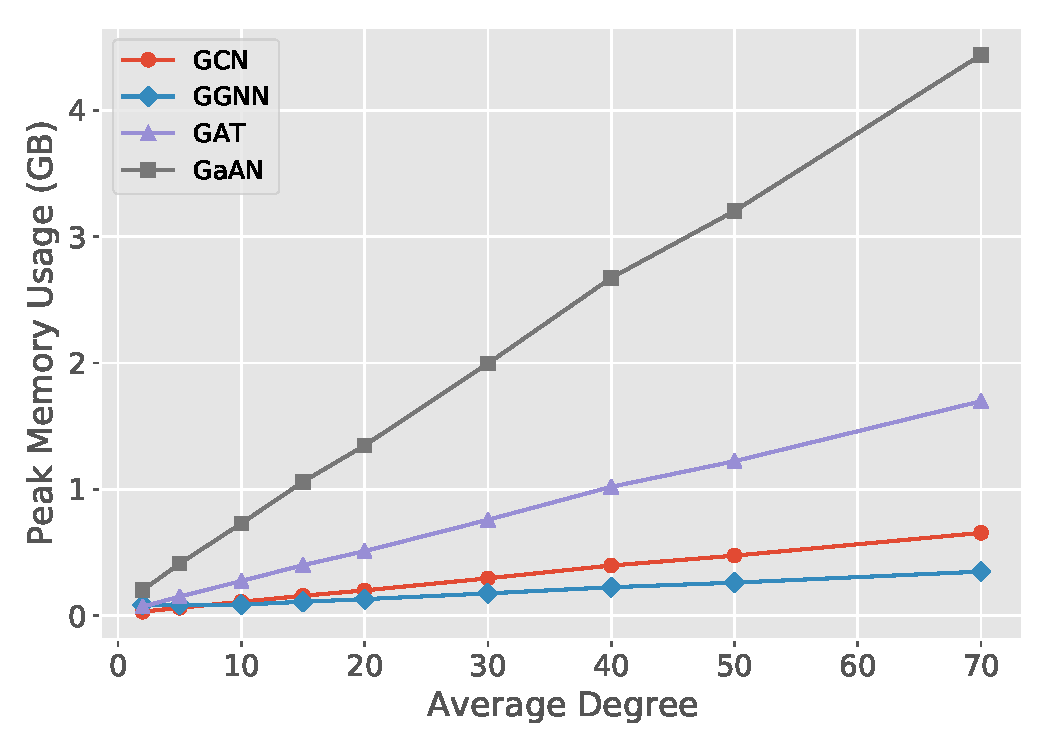
\includegraphics[height=4cm]{figs/experiments/exp_memory_expansion_ratio_input_graph_number_of_edges_peak_memory.pdf}}
    \subfloat[Memory expansion ratio]{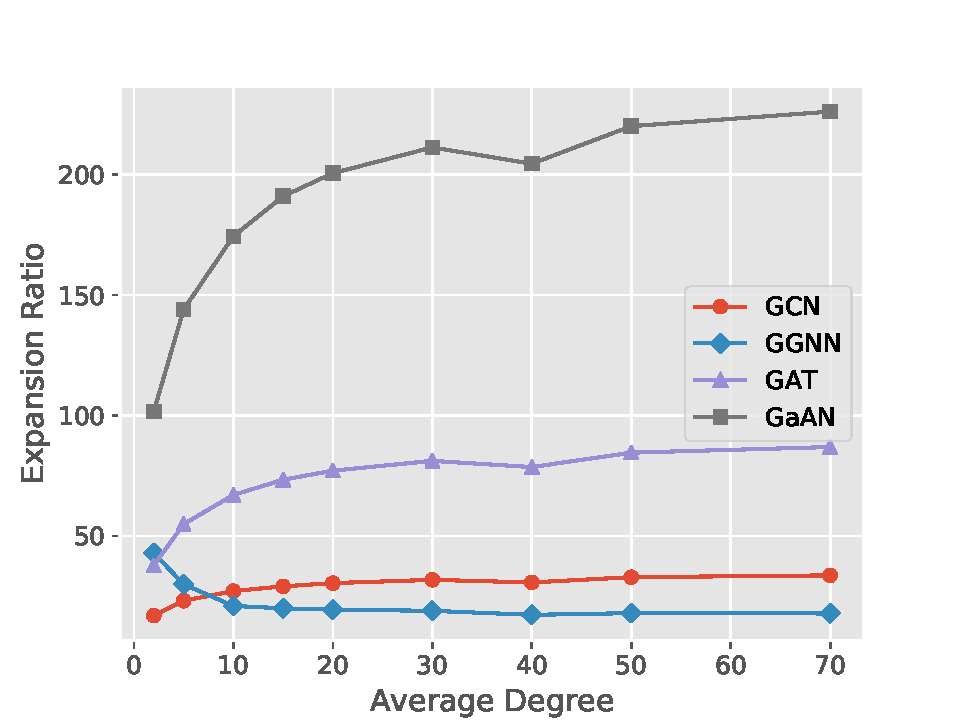
\includegraphics[height=4cm]{figs/experiments/exp_memory_expansion_ratio_input_graph_number_of_edges_expansion_ratio.pdf}}
    \caption{Memory usage under different average degrees. The random graphs were generated by fixing the number of vertices at 10K and the dimension of input feature vectors at 32.}
    \label{fig:exp_memory_expansion_ratio_input_graph_number_of_edges}
\end{figure}

We also fixed the number of edges $|\mathcal{E}|$ and generated random graphs with different $|\mathcal{V}|$.
%
\figurename~\ref{fig:exp_memory_expansion_ratio_input_graph_number_of_vertices_fixed_edge} shows how the memory usage changed according to $|\mathcal{V}|$.
%
MERs of all GNNs were insensitive to $|\mathcal{V}|$, compared to $|\mathcal{E}|$.
%
Except for GGNN, the MERs of the other GNNs declined as $|\mathcal{V}|$ increased because the sizes of the datasets increased more quickly than the sizes of the intermediate results.
%
As GGNN had high vertex calculation complexity, the sizes of the intermediate results were very sensitive to $|\mathcal{V}|$.
%
It indicated that \emph{the intermediate results of the edge calculation stage dominated the memory usage during the GNN training}.

\begin{figure}[H]
    \centering
    \subfloat[Peak memory usage]{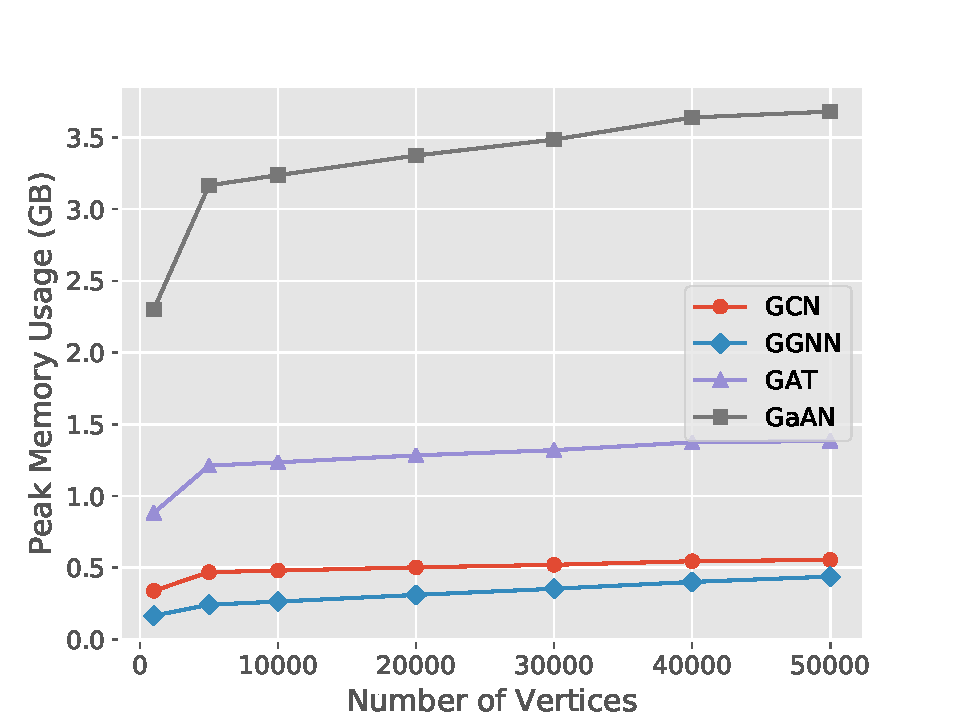
\includegraphics[height=4cm]{figs/experiments/exp_memory_expansion_ratio_input_graph_number_of_vertices_fixed_edge_peak_memory.pdf}}
    \subfloat[Memory expansion ratio]{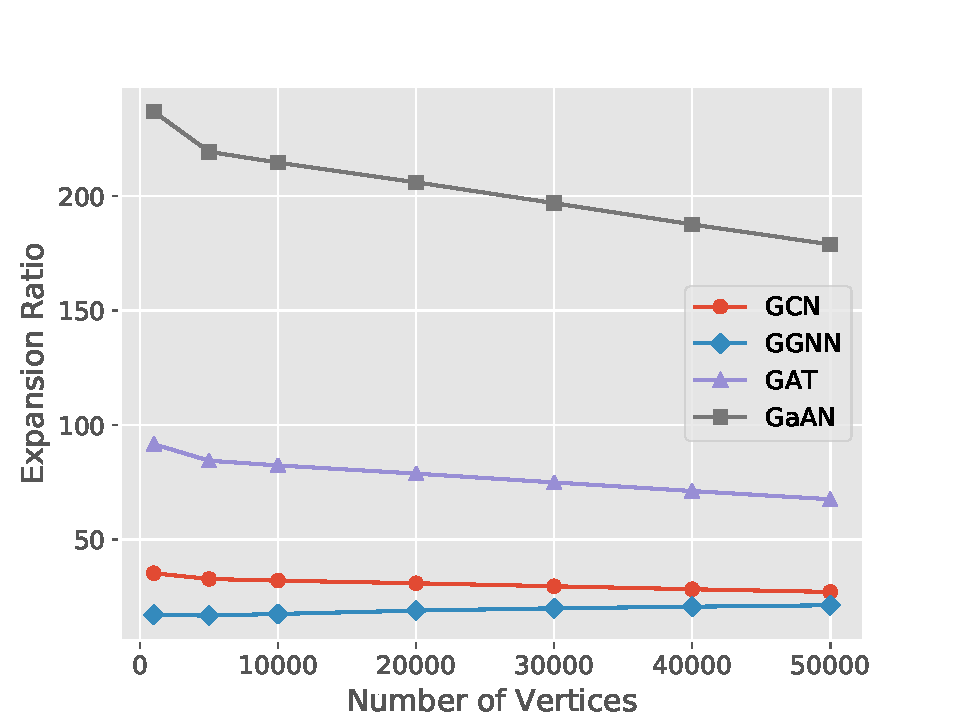
\includegraphics[height=4cm]{figs/experiments/exp_memory_expansion_ratio_input_graph_number_of_vertices_fixed_edge_expansion_ratio.pdf}}
    \caption{Memory usage under different numbers of vertices. The random graphs were generated by fixing the number of edges at 500K and the dimension of input feature vectors at 32.}
    \label{fig:exp_memory_expansion_ratio_input_graph_number_of_vertices_fixed_edge}
\end{figure}

\paragraph{Summary of Memory Usage}
%
The \emph{high} memory expansion ratio severely restricted the data scalability of GNN training.
%
The memory usage mainly came from the intermediate results of the \emph{edge calculation stage}.
%
Fixing the number of vertices, the memory usage increased \emph{linearly} along with the number of edges.
%
Fixing the GNN structure and the hyper-parameters, increasing the dimension of input feature vectors could reduce the memory expansion ratio.
%
To reduce the memory usage of GNN training, optimizations should focus on reducing memory footprints of the edge calculation stage.

\subsection{Effects of Sampling Techniques on Performance}
\label{sec:effects_of_sampling_techniques_on_performance}

With the sampling techniques, GNNs were trained in a mini-batch manner.
%
Each mini-batch updated the model parameters based on a small subgraph sampled from the original input graph.
%
Thus, the training time per batch and the peak memory usage during the training both declined significantly.

In the implementation in PyG, the GNN model and the dataset resided on the GPU side.
%
To process each epoch, PyG sampled the original dataset in the main memory and generated several batches.
%
Each batch was a small subgraph of the dataset.
%
To train on each batch, PyG sent the sampled subgraph to the GPU, calculated the gradients on the subgraph, and updated the model parameters directly on the GPU.
%
With the sampling techniques, the model parameters were updated by a stochastic gradient descent optimizer.
%
PyG conducted the evaluation phase every several epochs or batches (either on the CPU side or the GPU side) to determine whether to stop the training.
%
In this section, the experiments focused on the training phase of each batch.

\figurename~\ref{fig:exp_sampling_minibatch_graph_info} shows how the size of the sampled subgraph changed with the batch size.
%
For the neighbor sampler, the relative batch size was the proportion of the sampled vertices of the last GNN layer in $\mathcal{V}$.
%
For the cluster sampler, the relative batch size was the proportion of the sampled partitions in all partitions of the graph.
%
The neighbor sampler was very sensitive to the batch size.
%
As the batch size increased, the size of the sampled subgraph first increased quickly and then stabilized.
%
The cluster sampler was much less sensitive compared to the neighbor sampler.
%
The number of vertices and the average degree of the sampled subgraphs increased linearly with the batch size.

\begin{figure}[H]
    \centering
    \subfloat[Neighbor sampler]{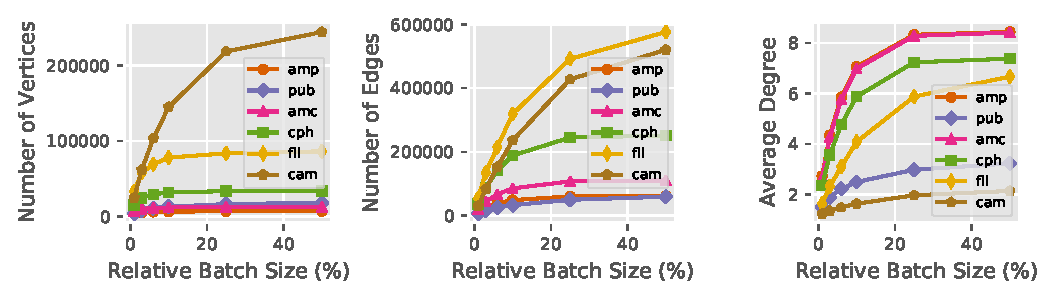
\includegraphics[height=4cm]{figs/experiments/exp_sampling_minibatch_realtive_graph_info_graphsage_gcn.pdf}} \\
    \subfloat[Cluster sampler]{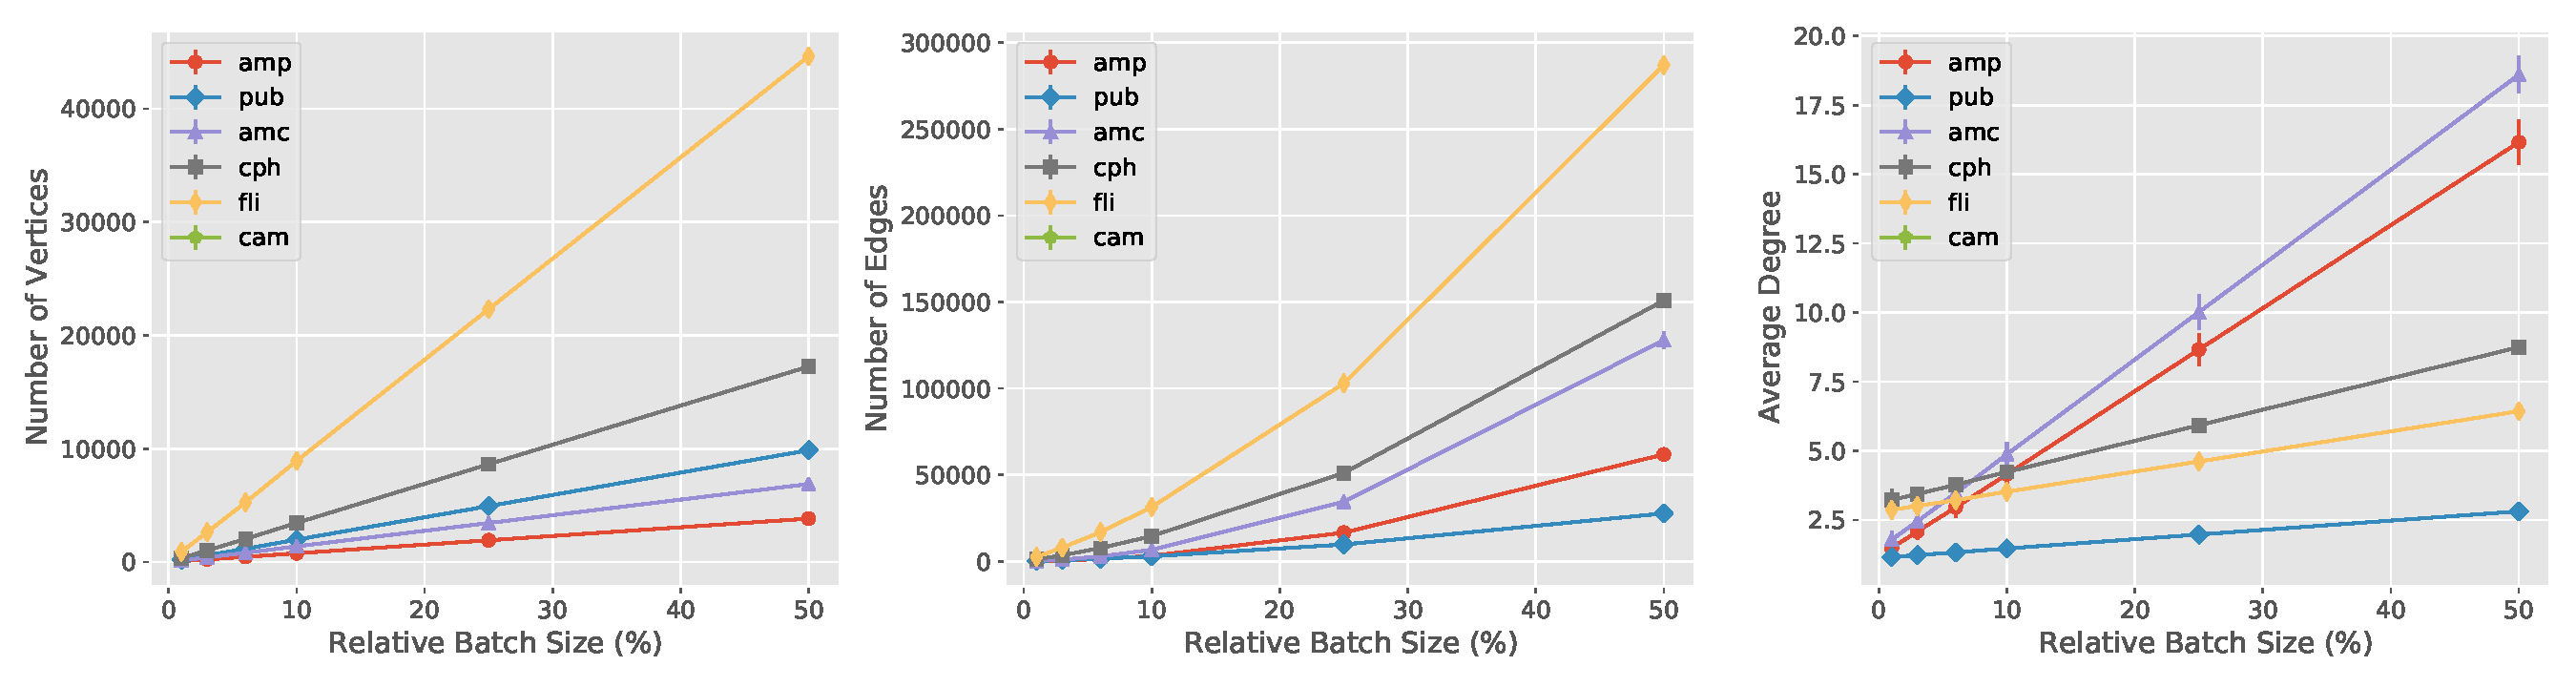
\includegraphics[height=4cm]{figs/experiments/exp_sampling_minibatch_realtive_graph_info_cluster_gcn.pdf}}
    \caption{Sizes of sampled subgraphs under different relative batch sizes. The batch size was relative to the full graph. Each batch size was sampled 50 times and the average values were reported. The error bar indicates the standard deviation.}
    \label{fig:exp_sampling_minibatch_graph_info}
\end{figure}

The average degree of the sampled subgraph was \emph{much lower} than the average degree of the original graph, especially when the relative batch size is low.
%
Taking the neighbor sampler with the relative batch size of 6\% as an example, the average degree of the \texttt{amp} dataset was 31.1, but the average degree of the sampled subgraph was only 5.8.
%
For the cluster sampler, the average degree was 3.0.
%
\figurename~\ref{fig:exp_sampling_minibatch_degrees_distribution} compares the degree distribution of the sampled subgraphs with the original graph.
%
The slopes of the curves were similar, indicating that the sampled subgraphs still followed the power-law degree distribution.
%
However, the numbers of high-degree vertices were much less than the original graph, lowering the average degrees.
%
According to the experimental results in Section~\ref{sec:training_time_breakdown}, if the average degree became lower, the proportion of the training time spent on the vertex calculation stage would become higher, especially for GGNN.

\begin{figure}[H]
    \centering
    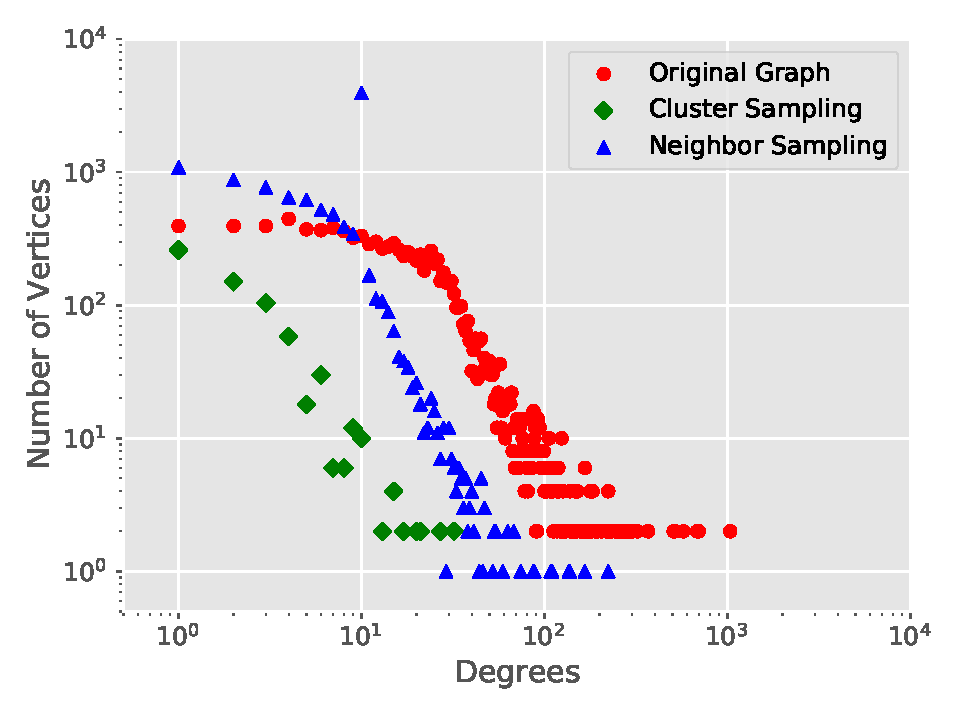
\includegraphics[width=0.4\columnwidth]{figs/experiments/exp_sampling_minibatch_degrees_distribution_amazon-photo.pdf}
    \caption{Vertex degree distribution of the sampled subgraph (relative batch size: 6\%) and the original graph. Dataset:\texttt{amp}.}
    \label{fig:exp_sampling_minibatch_degrees_distribution}
\end{figure}

To find out performance bottlenecks of the sampling techniques, we decomposed the training time per batch into three phases: \emph{sampling} on the CPU side, \emph{transferring} sampled subgraphs from the CPU side to the GPU side, and \emph{training} with the sampled subgraphs on the GPU side.
%
\figurename~\ref{fig:exp_sampling_batch_train_time} shows the time breakdown of the four GNNs under different relative batch sizes.
%
For the neighbor sampler, the sampling technique reduced the training time per batch only when the batch size was very small.
%
When the batch became bigger, the sampling and the data transferring phases introduced noticeable overheads, making the training time exceed the full-batch training.
%
For the clustering sampler, the sampled subgraph was smaller than the neighbor sampler under the same relative batch size.
%
The reduction in the training time was more obvious than the neighbor sampler.
%
However, the overheads increased quickly as the relative batch size increased.
%
The training time under the 25\% relative batch size already exceeded the time of full-batch training.
%
The experimental results indicated that the current implementation of the sampling techniques in PyG was inefficient.
%
When the batch size was large, more than 50\% of the time had been spent on sampling and data transferring.
%
\emph{The sampling techniques were only efficient under small batch sizes.}


\begin{figure}[H]
    \centering
    \subfloat[Neighbor sampler on \texttt{amc}]{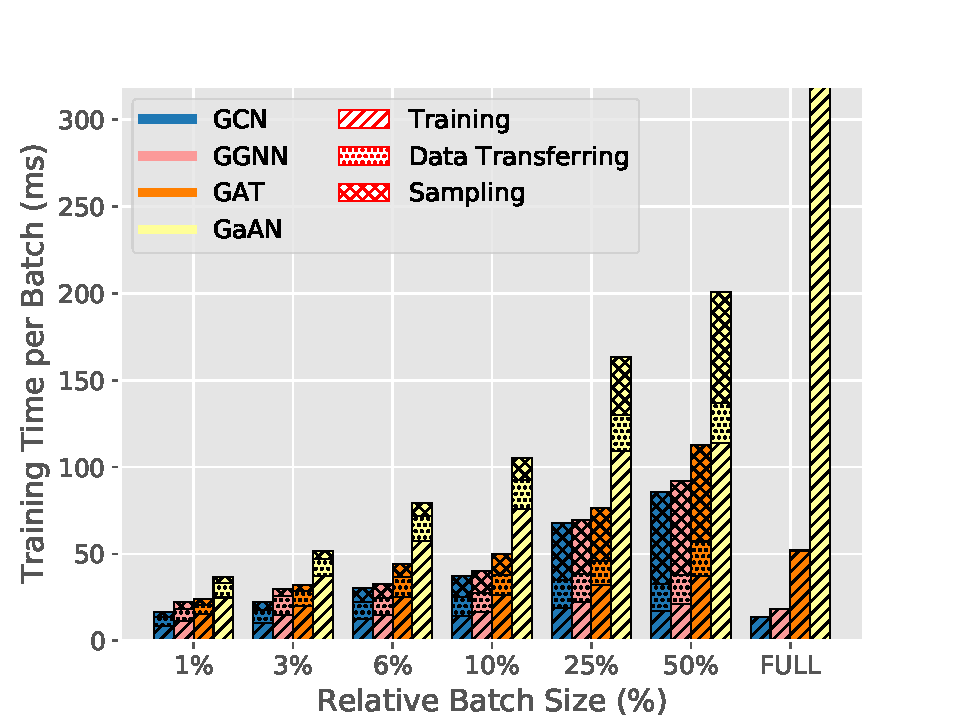
\includegraphics[height=5cm]{figs/experiments/exp_sampling_relative_batch_size_train_time_stack_graphsage_amazon-computers.pdf}}
    \subfloat[Neighbor sampler on \texttt{fli}]{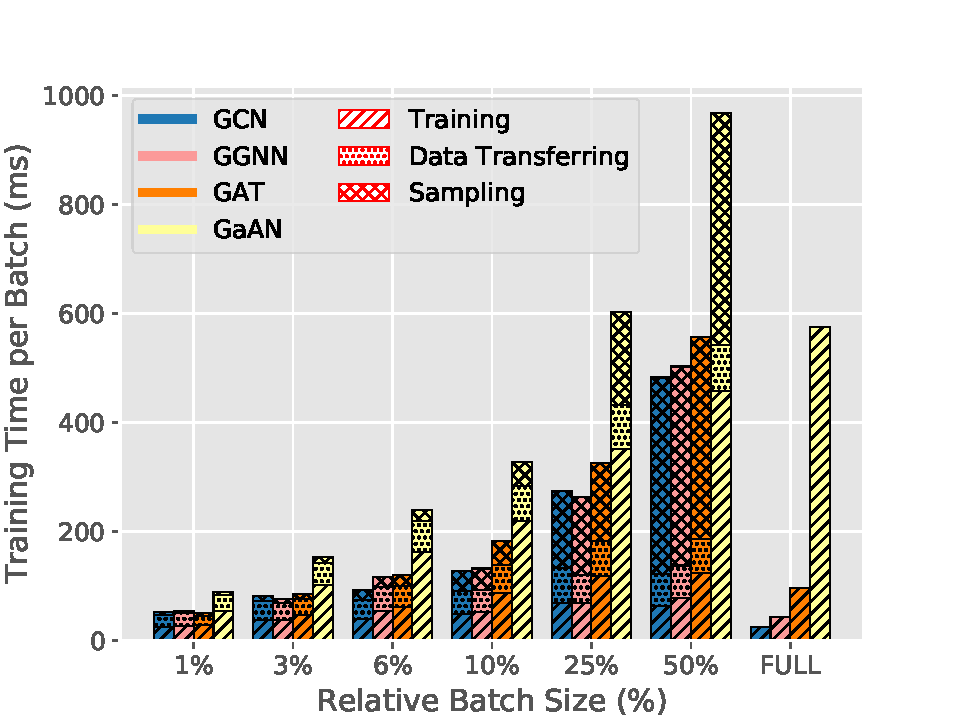
\includegraphics[height=5cm]{figs/experiments/exp_sampling_relative_batch_size_train_time_stack_graphsage_flickr.pdf}} \\
    \subfloat[Cluster sampler on \texttt{amc}]{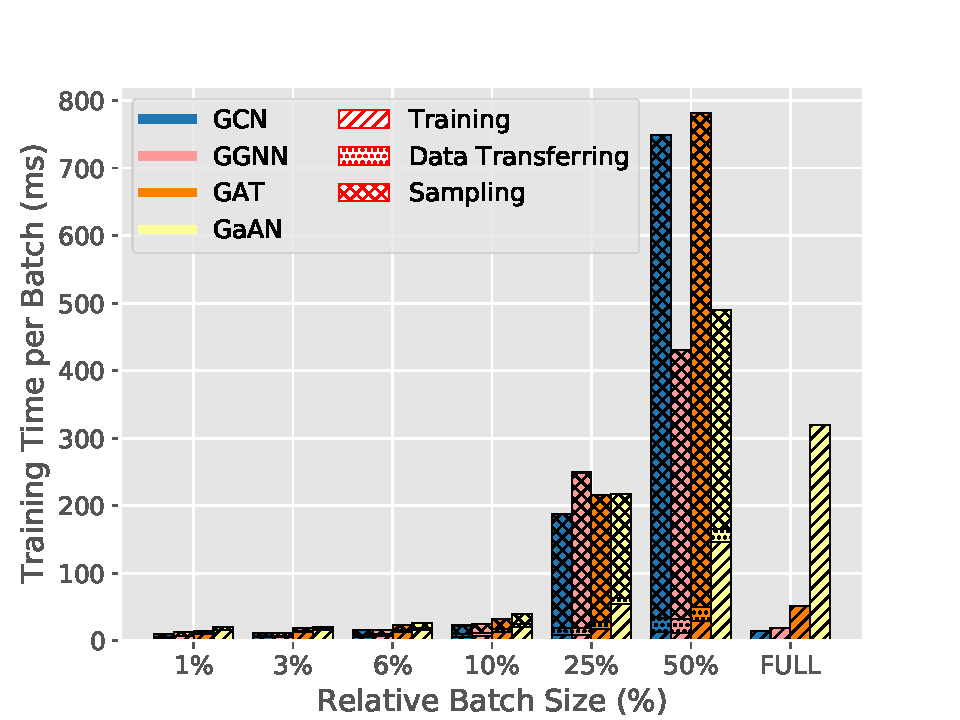
\includegraphics[height=5cm]{figs/experiments/exp_sampling_relative_batch_size_train_time_stack_cluster_amazon-computers.pdf}}
    \subfloat[Cluster sampler on \texttt{fli}]{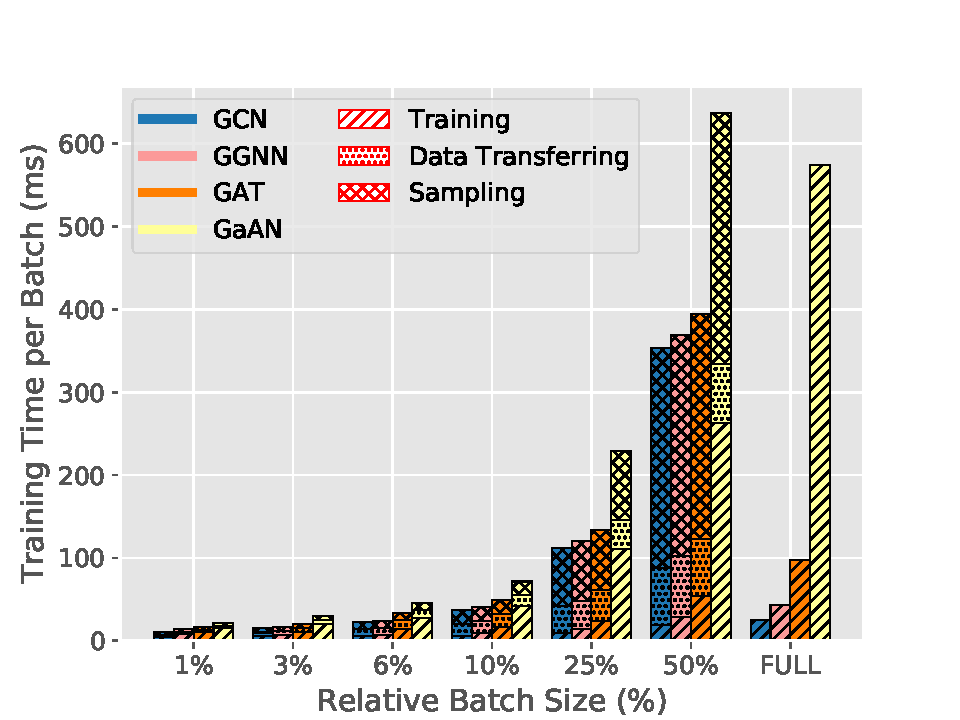
\includegraphics[height=5cm]{figs/experiments/exp_sampling_relative_batch_size_train_time_stack_cluster_flickr.pdf}}
    \caption{Training time per batch breakdown. FULL means that the full graph participates in the training.}
    \label{fig:exp_sampling_batch_train_time}
\end{figure}

The main advantage of the sampling techniques was \emph{reducing the peak memory usage} during training.
%
\figurename~\ref{fig:exp_sampling_memory_usage} shows the memory usage under different batch sizes.
%
The peak memory usage declined significantly even under big batch sizes.
%
The sampling techniques made training GNNs on big graphs \emph{possible} for GPUs.

\begin{figure}[H]
    \centering
    \subfloat[Neighbor sampler on \texttt{amc}]{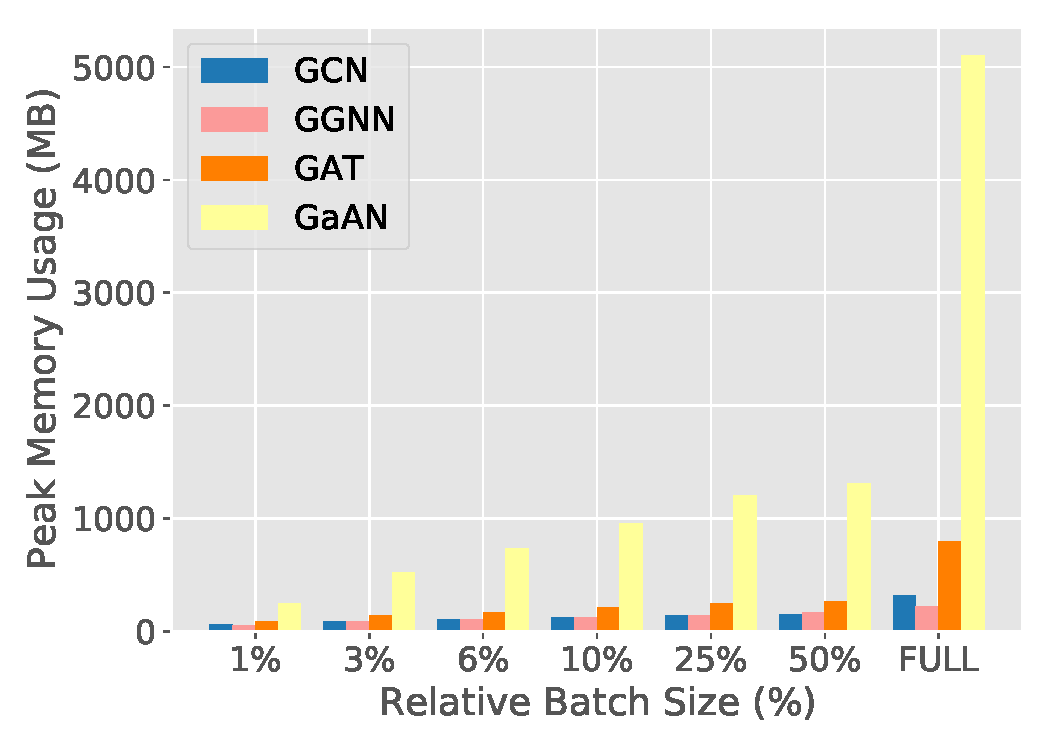
\includegraphics[height=4cm]{figs/experiments/exp_sampling_memory_usage_relative_batch_size_graphsage_amazon-computers_peak_memory.pdf}}
    \subfloat[Neighbor sampler on \texttt{fli}]{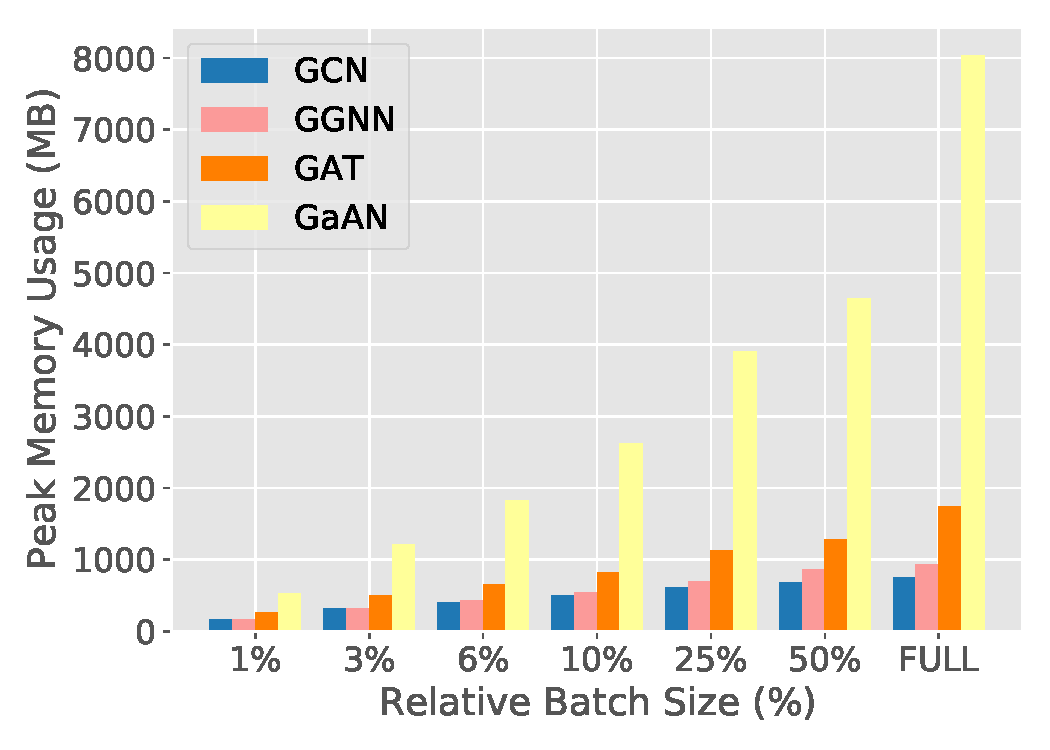
\includegraphics[height=4cm]{figs/experiments/exp_sampling_memory_usage_relative_batch_size_graphsage_flickr_peak_memory.pdf}} \\
    \subfloat[Cluster sampler on \texttt{amc}]{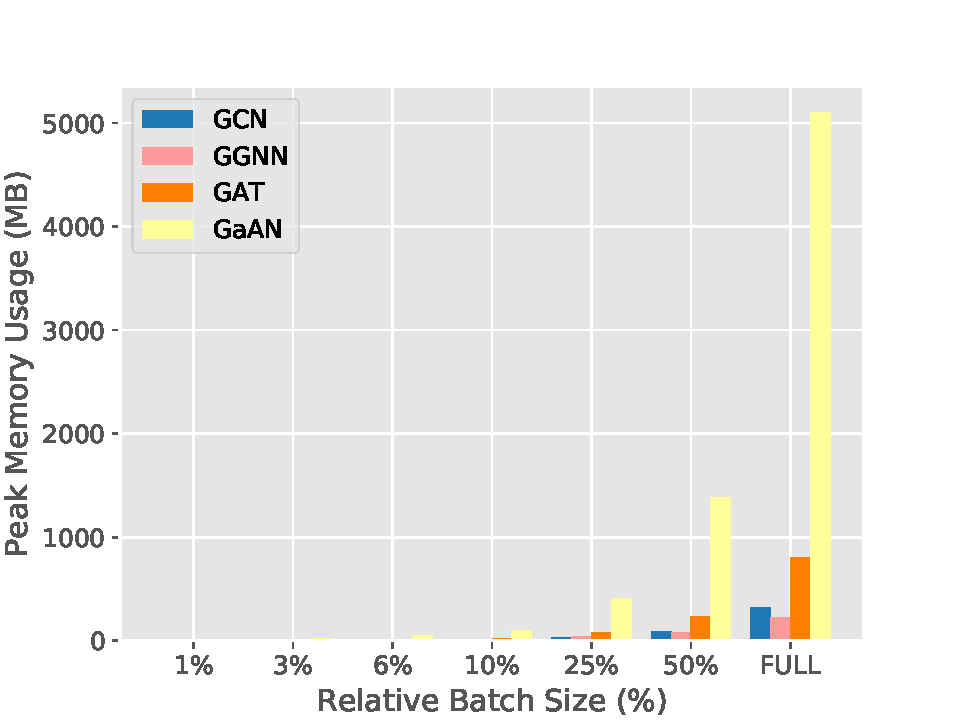
\includegraphics[height=4cm]{figs/experiments/exp_sampling_memory_usage_relative_batch_size_cluster_amazon-computers_peak_memory.pdf}}
    \subfloat[Cluster sampler on \texttt{fli}]{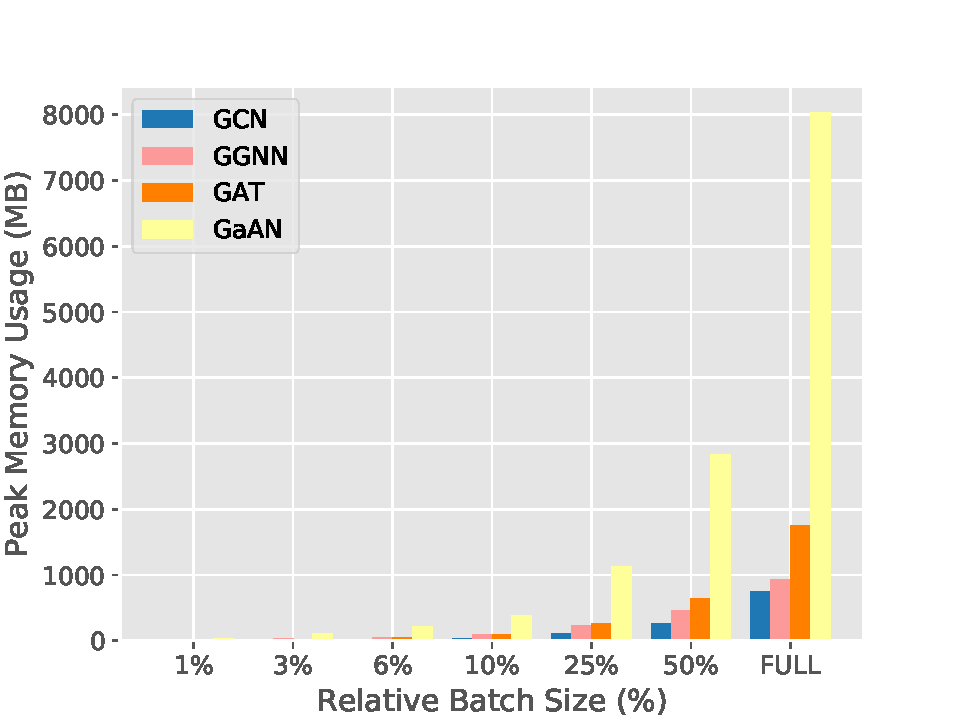
\includegraphics[height=4cm]{figs/experiments/exp_sampling_memory_usage_relative_batch_size_cluster_flickr_peak_memory.pdf}}
    \caption{Peak memory usage under different batch sizes. FULL means that the full graph participated in the training.}
    \label{fig:exp_sampling_memory_usage}
\end{figure}

The disadvantage of the sampling technique was wasting GPU resources.
%
As the sampling techniques were only effective under small batch sizes, the sampled subgraphs were very small in those cases.
%
They could not make full use of the computing power of a GPU.
%
To simulate the situation, we generated random graphs with few vertices and measured the training time per batch in \figurename~\ref{fig:exp_small_graph_train_time}.
%
As the number of vertices increased, the training time was almost unchanged except for GaAN.
%
The training time of GaAN increased only with $|\mathcal{V}| \geq 4000$.

\begin{figure}[H]
    \centering
    \includegraphics[height=5cm]{figs/experiments/exp_small_graph_train_time.pdf}
    \caption{Training time per epoch on small random graphs. For each number of vertices, we generated 50 random graphs with the average degree of 4.0 and reported the average training time per batch (without the evaluation phase). The error bar indicates the standard deviation.}
    \label{fig:exp_small_graph_train_time}
\end{figure}


\paragraph{Summary of Sampling Techniques}

The sampled subgraphs had lower average degrees than the original graph.
%
With small batch sizes, the sampling techniques could significantly reduce the training time per batch and the peak memory usage.
%
However, small batch sizes could not make full use of the computing power of a GPU.
%
With big batch sizes, the current implementation of the sampling techniques in PyG was inefficient.
%
The time spent on the sampling phase and the data transferring phase even exceeded the training phase.
